\chapter{Graph Isomorphism}
\label{ch:iso}

\begin{abstract}
  Subgraph isomorphism is a fundamental property of graphs that
  requires checking whether the network structure of one graph can be
  found (embedded) within another graph.  It has numerous applications
  and is a computationally challenging problem: it is NP-complete and
  known algorithms explore an exponentially large search space.  Even
  though it has been studied extensively, relatively little is known
  about whether subgraph isomorphism accepts a parallel solution.  In
  this paper, we present a parallel algorithm for subgraph (and graph)
  isomorphism problem.  We describe the algorithm, prove its key
  correctness and efficiency properties, including its work
  efficiency, and present an implementation targeting modern multicore
  machines. We perform an empirical evaluation by considering a
  publicly available graph benchmarking suite. Our results show that
  the algorithm achieves good performance and scalability up to 70
  cores.

\end{abstract}


%% \begin{abstract}
%% The graph and subgraph isomorphism problems require checking whether
%% two directed graphs and are entirely isomorphic, i.e., encode the same
%% network structure, or if one in isomorphic to a subgraph of
%% another.
%% %%
%% %% Recent results by Babai has shown that graph isomorphism accepts a
%% %% quasi-polynomial algorithm, though as claimed by Babai, the algorithm
%% %% is not practical.
%% %% %
%% %% The more general subgraph-isomorphism problem requires finding a
%% %% subgraph of a graph that is isomorphic to the another graph.
%% %% %
%% %% Subgraph isomorphism is NP-complete.
%% %%
%% Subgraph isomorphism is an NP-complete problem, whereas recent results
%% by Babai show graph isomorphism to be quasi-polynomial.
%% %

%% Even though both problem are difficult, they are important in practice
%% and thus there has been much work on designing and implementing
%% practical algorithms.
%% %
%% These algorithms typically perform a search in a very large search
%% space and require exponential time in the worst case.
%% %
%% They can, however, work reasonably efficiently on small to moderate
%% graphs (usually consisting of 1000's of nodes).
%% %
%% Nearly all existing graph and subgraph isomorphism algorithms are
%% sequential.

%% In this paper, we present a parallel algorithm for the problem of
%% subgraph (and graph) isomorphism.
%% %
%% We describe the algorithm, prove some key correctness and efficiency
%% properties and present an implementation.
%% %
%% We perform an empirical evaluation of our algorithm by considering a
%% publicly available graph benchmarking suite of more than thousand
%% graphs.
%% %
%% Our results show that the algorithm achieves good performance and
%% scalability.
%% %
%% \end{abstract}

%% % space overhead is p*n + p*n^2 - because at level only n things at most, and at most
%% % n levels per processor

%\documentclass[12pt]{article}
\usepackage{../template/lect}
\usepackage{../template/code}
\usepackage{tabularx}
\usepackage{booktabs}
\usepackage{colortbl}
\usepackage{graphicx,xcolor,lipsum}
\usepackage{titlesec}



%\usepackage[svgnames]{xcolor}
\usepackage{tikz}
\usetikzlibrary{shapes,snakes}
%\usepackage{tkz-graph}

\addtolength{\parskip}{7pt}


\Lecturer{\umut}
\LectureNumber{1}
\LectureDate{August 27, 2013}
\LectureVersion{2.0}
\LectureTitle{Overview and Sequencing the Genome}

% \newenvironment{optional}{
% \begin{tikzpicture}
%   \node[fill=gray!20,rectangle,inner sep=10pt](box) {
%     \begin{minipage}{0.96\textwidth}
% }{\end{minipage}
%  };
% \end{tikzpicture}}

\usepackage{microtype}
\renewcommand{\topfraction}{1.0}	% max fraction of floats at top
\renewcommand{\bottomfraction}{1.0}	% max fraction of floats at bottom
\renewcommand{\textfraction}{0.1}

\begin{document}
%% Change this to derive notes for different levels.
%% Use one of the following 
%% \levelLectureNotes to include everything
%% \levelLectureSummaryE, to include easy stuff
%% \levelLectureSummaryM, to include moderate stuff
%% \levelLectureSummaryD to include difficult stuff
%% \levelLectureSummary to exclude all questions and level-qualified figures and such.
 
%\renewcommand{\compilationLevel}{\levelLectureNotes} % the notes for the students
%\renewcommand{\compilationLevel}{\levelLectureSummaryE} % intermediate
%\renewcommand{\compilationLevel}{\levelLectureSummaryM} % intermediate
\renewcommand{\compilationLevel}{\levelLectureSummary} % summary
%\renewcommand{\compilationLevel}{\levelLecture}  % for lecture delivery


\MakeScribeTop



\chapter{Probability Theory}
\label{ch:probability}
{ 

\newcommand{\qsort}{quicksort}
\newcommand{\Qsort}{Quicksort}


\newcommand{\SSpace}{\ensuremath{\Omega}}
\newcommand{\EventE}{\mathcal{E}}

We present a brief review of basic discrete probability theory that we
shall use in this book.
%
The  chapter is organized into three sections.  In the first section,
we describe probabilistic models, events, probabilities and
conditional probabilities. 
%
In the second section, we describe random variables, which correspond
closely with events, because as events, they can be thought as
assigning probabilities to subsets of the sample space.
%
The structure of this section follows that of the first section,
reflecting various forms of probability laws on events to random
variables.
%
In the third and final part, we describe expectations, which can be
used to summarize random variables by their average or mean value.
%


\section{Probabilistic Models}
\label{sec:probability}

Let's begin with an example.

\begin{example}
Suppose we have two \emph{fair} dice, meaning that each is equally
likely to land on any of its six sides.  If we toss the dice, what is
the chance that their numbers sum to $4$?  
%
You can probably figure out
that the answer is
\begin{equation*}
\frac
{\text{\# of outcomes that sum to}~4}
{\text{\# of total possible outcomes}} 
= 
\frac{3}{36} = \frac{1}{12}
\end{equation*}
since there are three ways the dice could sum to 4 (1 and 3, 2 and 2,
and 3 and 1), out of the $6 \times 6 = 36$ total possibilities.
\end{example}
%

Probability theory is a mathematical study of uncertain situations
such as the dice game in our example.
%
In probability theory, we think of a game such as our dice game as an
\defn{experiment}, because it is an ``experiment'' that we can repeat
to obtain a number of outcomes.

%
The idea behind probability theory is to use a \defn{probabilistic
  model} that models the situation in precise, mathematical terms.
%
A probability model consists of a \defn{sample space} and a
\defn{probability function}, also called \defn{probability law} that
satisfies certain axioms that we shall see.

\paragraph{Sample Spaces and Events.} 
A \defn{sample space} \SSpace{} is an arbitrary and possibly infinite
(but countable) set of possible outcomes of a probabilistic
experiment. 
%
For the dice game, the sample space is the 36 possible outcomes of the
dice.  
%
An \defn{event} is any subset of $\SSpace$ and
most often representing some property common to multiple outcomes.  
%
We typically denote events by capital letters from the start
of the alphabet, e.g. $A$, $B$, $C$.


\begin{definition}[Probabilistic Model]
  A probabilistic model for an experiment consists of a \defn{sample
    space} that represents the outcomes of that experiment and a
  \defn{probability law} or   \defn{probability function} that assigns to an event $A$ a value
  representing the likelihood of that event occurring.

Probability law must satisfy the following axioms.

\begin{itemize}
\item \textbf{Nonnegativitiy:} $\prob{A} \in [0,1]$.

\item \textbf{Additivity:} for any two disjoint events $A$ and $B$, $\prob{A \cup B} =
  \prob{A} + \prob{B}$.

\item \textbf{Normalization:} $\prob{\SSpace} = 1$.
\end{itemize}

\end{definition}

Note that when defining the probabilistic model, we have not specified
carefully what kinds of events, we may be interested in, because they
may differ based on the experiment and what we are interested in.
%
We do, however, must take care when setting up the probabilistic model
to reason about the experiment correctly. 
%
For example, each element of the sample space must correspond to one
unique outcome of the experiment.  In other words, they must be
mutually exclusive. 
%
Similarly, any actual outcome of the experiment must have a
corresponding representation in the sample space.

When working with discrete probabilistic models, it is common practice
to consider each outcome on its own and assign to it a probability.
%
The probability for any event can then be computed by using the
additivity  property of the probability law and summing up the
probabilities of the outcomes constituting the event.

\begin{example}
  For our example of throwing two dice, the sample space
  consists of all of the $36$ possible pairs of values of the dice:
\[
\SSpace = \{(1,1),(1,2),\ldots,(2,1),\ldots,(6,6)\}.
\]
%
Each pair in the sample space corresponds to an outcome of the experiment.
%
The outcomes are mutually exclusive and cover all possible outcomes of
the experiment.


For example, having the first dice show up $1$ and the second $4$ is
an outcome and corresponds to  the element $(1,4)$ of the sample space $\Omega$.

The event that the ``the first dice is 3'' corresponds to the
set
\[
A = \csetf{(d_1,d_2) \in \Omega}{d_1 = 3} =
\{(3,1),(3,2),(3,3),(3,4),(3,5),(3,6)\}.
\]
The event that ``the dice sum to 4'' corresponds to the set
\[
B = \csetf{(d_1,d_2) \in \Omega}{d_1 + d_2 = 4} =
\{(1,3),(2,2),(3,1)\}.
\]

Assuming the dice are unbiased, the probability law over
the sample space can be written as 
\[
\prob{x} = 1/36.
\]

The probability of the event $A$ (that the first dice
is 3) is thus 
\[
\prob{A} = \sum_{x \in A} \prob{x} = \frac{6}{36} = \frac{1}{6}. 
\]

If the dice were biased so the probability that it shows up with a
particular value is proportional to the value, then the probability
function would be $\prob{(x,y)} = \frac{x}{21} \times \frac{y}{21}$,
and the probability of the event $B$ (that the dice add to 4) would be
\[
\prob{B} = \sum_{x \in B} \prob{x} = \frac{1 \times 3 + 2 \times 2
  + 3 \times 1}{21 \times 21} = \frac{10}{441}. 
\]

\begin{notesonly}
One way to do these sums in class is no note that (1 + ... + 6) is
repeated and it adds up to 21.
\end{notesonly}
\end{example}

\paragraph{Properties of Probability Laws.}

Given a probabilistic model, 
we can prove several properties of probability laws by using the
three axioms that they must satisfy.

For example, if for two events $A$ and $B$.  We have
\begin{itemize}
\item if $A \subseteq B$, then  $\prob{A} \le \prob{B}$,
\item $\prob{A \cup B} = \prob{A}  + \prob{B} -  \prob{A \cap B}$.
\end{itemize}

\paragraph{The Union Bound.}  

The union bound, also known as Boole's inequality, is a simple way to
obtain an upper bound on the probability of any of a collection of events
happening.  Specifically for a collection of events
$A_0, A_2, \ldots, A_{n-1}$ the bound is:
\[
\prob{\bigcup_{0 \leq i < n} A_i} \leq \sum_{i=0}^{n-1} \prob{A_i} 
\]
This bound is true unconditionally.
%
To see why the bound holds we note that the primitive events
in the union on the left are all included in the sum on the right
(since the union comes from the same set of events).  
%
In fact they
might be included multiple times in the sum on the right, hence the
inequality.  In fact sum on the right could add to more than one, in
which case the bound is not useful.  
%
The union bound can be useful in generating high-probability bounds
for algorithms. For example, when the probability of each of $n$
events is very low, e.g. $1/n^5$ and the sum remains very low,
e.g. $1/n^4$.



\paragraph{Conditional probability}


Conditional probability allows us to reason about dependencies between
observations.  
%
For example, suppose that  your friend rolled a pair of dice and told
you that they sum up to $6$, what is the probability that the one of
dice has come up $1$?  
%
Conditional probability has many practical applications in the real
world.  
%
For example, given that medical test for a disease comes up
positive, we might want to know  the probability that the patient has the disease. 
%
Or, given that your computer has been working fine for the past 2
years, you might want to know the probability that it will continue
working for one more year.



\begin{definition}
For a given probabilistic model consisting of a sample space and
probability function, we define the conditional probability of an
event $A$ given $B$, as the probability of $A$ occurring given that
$B$ occurs as 
\[
\prob{A \given B} = \frac{\prob{A \cap B}}{\prob{B}}. 
\]

The conditional probability measures the probability that the event
$A$ occurs given that $B$ does.  It is defined only when $\prob{B} > 0$.
\end{definition}

Conditional probability satisfies the three axioms of probability
laws and thus itself a probability law.
%
\begin{notesonly}
$\prob{A \given B} \ge 0$ holds because $\prob{A \cap B}$ is
nonnegative.

Given disjoint $A_0$ and $A_1$.
\[
\begin{array}{lll}

\prob{(A_0 \cup A_1) \given B} & = & \prob{(A_0 \cup A_1) \cap B)} /
\prob{B}
\\[2mm]
& = & \prob{(A_0 \cap B) \cup (A_1 \cap B)} / \prob{B}
\\
& = & \prob{(A_0 \cap B)} / \prob{B} +  \prob{(A_1 \cap B) \mbox(by
  additivity because the two sets are disjoint}
\\
& = & ...
\end{array}
\]
The final property holds trivially because $\SSpace \cap B = B$. 

Thus conditional probabilities simple mass probabilities over the
event $B$ that we are interested in. 

\end{notesonly}

%
We can thus treat conditional probabilities just as ordinary
probabilities.  Intuitively, conditional probability can be thought as
a focusing and re-normalization of the probabilities on the
assumed event $B$.
%


\begin{example}
Consider throwing two fair dice and calculate the probability that the
first dice comes us $1$ given that the sum of the two dice is $4$. 
%
Let $A$ be the event  that the first dice comes up $1$ and $B$ the
event that the sum is $4$.
%
We can write $A$ and $B$ in terms of outcomes as 
\[
\begin{array}{lll}
A & = & \{ (1,1), (1,2), (1,3), (1,4), (1,5), (1,6) \}~\mbox{and}
\\
B & = & \{ (1,3), (2,2), (3,1) \}.
\end{array}
\]
We thus have $A \cap B = \{ (1,3) \}$.
%
Since each outcome is equally likely, 
\[
\prob{A \given B} = \frac{\prob{A \cap B}}{\prob{B}} 
%
= 
%
\frac{|A \cap B|}{|B|} = \frac{1}{3}.
\]
\end{example}

\begin{example}
Consider throwing two fair dice and calculate the probability that the
first dice comes up $1$ given that the second dice comes up $2$. 
%
Let $A$ be the event  that the first dice comes up $1$ and let $B$ the
event that the second dice comes up $2$.
%
We can write $A$ and $B$ in terms of outcomes as 
\[
\begin{array}{lll}
A & = & \{ (1,1), (1,2), (1,3), (1,4), (1,5), (1,6) \}~\mbox{and}
\\
B & = & \{ (1,2), (2,2), (3,2), (4,2), (5,2), (6,2) \}~\mbox{and}
\end{array}
\]
We thus have $A \cap B = \{ (1,2) \}$.
%
Since each outcome is equally likely, 
\[
\prob{A \given B} = \frac{\prob{A \cap B}}{\prob{B}} 
%
= 
%
\frac{|A \cap B|}{|B|} = \frac{1}{6}.
\]

Since $\prob{A} = \frac{|A|}{|\SSpace|} = \frac{1}{6}$, we have
concluded that $\prob{A \given B} = \prob{A}$, that is $A$ is
independent of $B$.  We shall see more about independence later in this
section.

\end{example}


\paragraph{Total Probability Law.}
Conditional probabilities can be useful in estimating the probability
of an event that may depend on a selection of choices.
%
The total probability theorem can be handy in such circumstances.

\begin{theorem}[Total Probability Law]
Consider a probabilistic model with sample space $\SSpace$ and let
$A_0, \ldots, A_{n-1}$ be a partition of $\SSpace$ such that $\prob{A_i} >
0$ for all $0 \le i < n$. 
%
For any event $B$ the following holds
\[
\begin{array}{lll}
\prob{B} 
& = & 
\prob{B \cap A_0} + \prob{B \cap A_1} + \ldots + \prob{B \cap A_{n-1}}
\\
& = & 
\prob{A_0}\prob{B  \given A_0} + \prob{A_1}\prob{B \given A_1} + \ldots + \prob{A_{n-1}}\prob{B \given A_{n-1}}
\end{array}
\]
\end{theorem}

\begin{example}
Your favorite social network partitions your connections into two
kinds, near and far.
%
The social network has calculated that the probability that you react
to a post by one of your far connections is $0.1$ but the same
probability is $0.8$ for a post by one of your near connections.
%
Suppose that the social network shows you a post by a near and far
connection with probability $0.6$ and $0.4$ respectively. 
%

Let's calculate the probability that you react to a post that you see
on the network.
%
Let $A_0$ and $A_1$ be the event that the post is near and far
respectively.
%
We have $\prob{A_0} = 0.6$ and   $\prob{A_1} = 0.4$.
%
Let $B$ the event that you react, we know that  $\prob{B \given A_0} =
0.8$ and $\prob{B \given A_1} = 0.1$.
%

We want to calculate $\prob{B}$, which by total probability theorem we
know to be 
\[
\begin{array}{lll}
\prob{B} 
& = &   \prob{B \cap A_0} + \prob{B \cap  A_1} 
\\
& = &  \prob{A_0}\prob{B \given A_0} + \prob{A_1}\prob{B \given  A_1}. 
\\
& = &  0.6 \cdot 0.8 +  0.4 \cdot 0.1
\\
& = &  0.52.
\end{array}
\] 

\end{example}

\begin{comment}

\paragraph{Bayes' Rule and Inference}

An important application of conditional probabilities is \defn{Bayes'
  Rule}, which can be stated as follows.
%
For any event $A$ and $B$ such that $\prob{B} > 0$, 
\[
\prob{A \given B} 
= 
\frac
{\prob{A} \prob{B \given A}}
{\prob{B}}.
\]
%
Bayes' rule follows easily by the definition of conditional
probability, because $\prob{A} \prob{B \given A} = \prob{A \cap B}$.

The importance of Bayes' rule is that it allows us to reverse the
direction of the conditional probability: when we are given the
probability of $B$ given $A$, we can infer the probability of $A$
given $B$.
%
This is sometimes referred as \defn{probabilistic inference}.


A common application of Bayes' Rule in the real world is inferring of
causes of an effect.  
%
More precisely, suppose that we observe an effect $B$ and we know the
probability that we would observe $B$ given $A$, i.e., $\prob{B \given
  A}$.
%
We want to know the probability that that the cause is indeed $A$,
i.e., $\prob{A \given B}$, which we can by using Bayes' Rule.

\begin{example}
We know that the probability of seeing smoke $B$ when there is fire
$A$ is $\prob{B \given A} = 0.9$ and that probability of seeing smoke
even when there is no fire is $\prob{B \given A^c} = 0.005$.
%
We also know independently that the probability
of having a fire at any time  is $\prob{A} = 0.001$.
%
Let's assume that we see some smoke and calculate the probability that
there is fire.
%
Let's consider the event $A^c$ that we don't see any fire, i.e., the
complement of $A$.  We have $\prob{A^c} = 0.009$. 
%
By using the total probability theorem, we have 
\[
\prob{B} = \prob{A} \prob{B | A} +  \prob{A^c} \prob{B | A^c}.
\]
This we can calculate as 
\[
\prob{B} = 0.001 \cdot  0.9 +  0.009 \cdot 0.005 = 0.000945
\]

%
By Bayes rule, we know that 
\[
\begin{array}{lll}
\prob{A \given B} 
& = &  
\frac
{\prob{A} \prob{B \given A}}
{\prob{B}}.
\\
& = & 
\frac
{0.001 \cdot 0.9}
{0.000945}
\\
& = & 0.953 
\end{array}
\]


\end{example}


\end{comment}








\paragraph{Independence.}

It is sometimes important to talk about the dependency relationship
between events.
%
Intuitively we say that two events are independent if  the occurrence
of one does not affect the probability of the other.
%
More precisely, we define independence as follows.  

\begin{definition}
Two events $A$ and $B$ are \defn{independent}   if 
\[
\prob{A \cap B} = \prob{A} \cdot \prob{B}.
\]  
%
We say that multiple events $A_0, \dots, A_{n-1}$  are \defn{mutually
  independent} if and only if, for any non-empty subset $I \subseteq \{0, \dots, n-1\}$,
\[
\prob{\bigcap_{i \in I} A_i} = \prod_{i\in I} \prob{A_i}.
\]
\end{definition}

Recall that  $\prob{A \given B} = \frac{\prob{A \cap
    B}}{\prob{B}}$ when $\prob{B} > 0$. Thus if $\prob{A \given B} = \prob{A}$ then
 $\prob{A \cap B} = \prob{A} \cdot \prob{B}$.
%
We can thus define independence in terms of conditional probability
but this works only when $\prob{B} > 0$. 



\begin{example}
For two dice, the events $A = \csetf{(d_1,d_2) \in
  \SSpace}{d_1=1}$ (the first dice is 1) and $B = \csetf{(d_1,d_2) \in
  \SSpace}{d_2=1}$ (the second dice is 1) are independent since
%
\[
\begin{array}{llccl}\
& \prob{A} \times \prob{B} & = & \frac{1}{6} \times \frac{1}{6} & = \frac{1}{36} \\[4mm]
= & \prob{A \cap B} & = & \prob{\cset{(1,1)}} & = \frac{1}{36}~.
\end{array}
\]
%
However, the event $C \equiv \event{X}{4}$ (the dice add to 4) is not independent of $A$
since 
\[
\begin{array}{llccl}
& \prob{A} \times \prob{C} & = &\frac{1}{6} \times \frac{3}{36} & = \frac{1}{72} \\[4mm]
\neq & \prob{A \cap C} & = & \prob{\cset{(1,3)}} & = \frac{1}{36}~.
\end{array}
\]
$A$ and $C$ are not
independent since the fact that the first dice is 1 increases the
probability they sum to $4$ (from $\frac{1}{12}$ to $\frac{1}{6}$).

\end{example}

\begin{simpleexample}
%% This is also a problem.

For two dice, let $A$ be the event that first roll is $1$ and $B$ be
the event that the sum of the rolls is $5$.
Show that they are independent.
\end{simpleexample}


\begin{simpleexample}
For two dice, let $A$ be the event that first roll is $1$ and $B$ be
the event that the sum of the rolls is $5$.

  Are these independent,
they turn out to be so.....

How about minimum is $2$ and so is the maximum?  They turn out not.

\end{simpleexample}

\begin{simpleexample}
Prove that disjoint events are never independent.
\end{simpleexample}

\section{Random Variables} 
A \defn{random variable} $X$ is a real-valued function on the outcomes
of an experiment, i.e., $X : \SSpace \to \R$, i.e., it assigns a real
number to each outcome.
%
For a sample space there can be many random variables, each keeping
track of some quantity of a probabilistic experiment.
%
We typically denote random variables by capital letters from
the end of the alphabet, e.g. $X$, $Y$, and $Z$.
%
We say that a random variable is \defn{discrete} if its range is
finite or countable infinite.  Throughout this book, we only consider
discrete random variables. 

\begin{example}
Consider rolling a dice.  The sample space is $\SSpace = \{1, 2, 3, 4,
5, 6 \}$.
%
We can define a random variable $X$ to map each primitive event to $0$
if the dice comes up an even number, or $1$ if the dice comes up an
odd number.
%
This random number is an indicator number indicating whether the dice
comes up an odd or an even number.
\end{example}

A random variable is called an \defn{indicator random variable} if it
takes on the value~$1$ when some condition is true and~$0$
otherwise.
%

For a random variable $X$ and a value $x \in \R$, we use the following
shorthand for the event corresponding to $X$ equaling $x$:
\[\event{X}{x} \equiv \csetf{y \in \SSpace}{X(y)  = x}~.\]


\begin{example}
For throwing two dice, we can define random variable as the sum of
the two dice:
\[
X(d_1,d_2) = d_1+d_2.
\]
We can define an indicator random variable
to getting doubles (the two dice have the same value):
\[
Y(d_1,d_2) =
\left\{
\begin{array}{ll}
1 & \mbox{if}~d_1 = d_2
\\
0 & \mbox{if}~d_1 \not= d_2
\end{array}
\right.
\]
Using our shorthand, the event $\event{X}{4}$ corresponds
to the event ``the dice sum to 4''.
\label{ex:rand::randvar}
\end{example}

\begin{remark}
The term random variable might seem counter-intuitive
since it is actually a function not a variable, and it is not really
random at all since it is a well defined deterministic function on the
sample space.  However if you think of it in conjunction with the
random experiment that selects a primitive element, then it is a
variable that takes on its value based on a random process.
\end{remark}

\paragraph{Probability Mass Function.}

For a discrete random variable $X$, we define its \defn{probability
  mass function} or \defn{PMF}, written $\pmf{X}(\cdot)$, for short as
a function mapping each element $x$ in the range of the random
variable to the probability of the event $\event{X}{x}$, i.e.,
\[
\pmf{X}(x) = \prob{\event{X}{x}}.
\]

\begin{example}
The probability mass function for the indicator random variable $X$
indicating whether the outcome of a roll of dice is comes up even is 
\[
\begin{array}{lll}
\pmf{X}(0) = \prob{\event{X}{0}} = \prob{\{1, 3, 5\}} =
1/2,~\mbox{and}
\\
\pmf{X}(1) = \prob{\event{X}{1}} = \prob{\{2, 4, 6\}} =
1/2.
\end{array}
\]

The probability mass function for the random variable $X$
that maps each outcome in a roll of dice to the smallest Mersenne
prime number no less than the outcome is
\[
\begin{array}{lll}
\pmf{X}(3) = \prob{\event{X}{3}} = \prob{\{1, 3\}} =
1/3,~\mbox{and}
\\
\pmf{X}(7) = \prob{\event{X}{7}} = \prob{\{2, 4, 5, 6\}} =
2/3.
\end{array}
\]
\end{example}

Note that much like a probability law, a probability mass function is
a non-negative function.
%
It is also additive in a similar sense: for any $x$ and $x'$, the
events $\event{X}{x}$ and $\event{X}{x'}$ are disjoint.
%
Thus for any set $\bar{x}$ of values of $X$, we have 
\[
\prob{X \in \bar{x}} = \sum_{x \in \bar{x}}{\pmf{X}(x)}.
\]
%
Furthermore, since $X$ is a function on the sample space, the events
corresponding to the different values of $X$ partition the sample
space, and we have
\[
\sum_{x}{\pmf{X}{x}} = 1.
\]
%
These are the important properties of probability mass functions: they
are non-negative, normalizing, and are additive in a certain sense. 


We can also compute the probability mass function for multiple random
variables defined for the same probabilistic model, i.e., same sample
space and probability law.
%
For example, the \defn{joint probability mass function} for two random
variables $X$ and $Y$, written $\pmf{X,Y}(x,y)$ denotes the
probability of the event $\event{X}{x} \cap \event{Y}{y}$, i.e.,
\[
\pmf{X,Y}(x,y) = \prob{\event{X}{x} \cap \event{Y}{y}} = \prob{X = x, Y = y}.
\]
%
Here
 $\prob{X = x, Y = y}$ is shorthand for   $\prob{\event{X}{x} \cap \event{Y}{y}}$.

Given joint probability mass function for a pair of random variables
$X$ and $Y$, we can calculate the probability mass function for any of
them, which is also called the \defn{marginal probability mass
  function} as follows
\[
\pmf{X}(x) = \sum_{y}{\pmf{X,Y}(x,y)},~\mbox{and}
\\
\pmf{Y}(y) = \sum_{x}{\pmf{X,Y}(x,y)}.
\]

In our analysis or randomized algorithms, we shall repeatedly
encounter a number of well-known random variables and create new ones
from existing ones by composition.

\paragraph{Bernoulli Random Variable.}
Suppose that we toss a  coin that comes up a head with probability $p$
and a tail with probability $1-p$.
%
The \defn{Bernoulli random variable} takes the value $1$ if the coin
comes up heads and $0$ if it comes up tails.
%
In other words, it is an indicator random variable indicating heads.
%
Its probability mass function is 
\[
\pmf{X}(x) = 
\left\{
\begin{array}{ll}
p & \mbox{if}~x = 1
\\
1-p & \mbox{if}~x = 0.
\end{array}
\right.
\]

\paragraph{Binomial Random Variable.}  

Consider $n$ Bernoulli trials with probability $p$.  We call the
random variable $X$ denoting the number of heads in the $n$ trials as
the \defn{Binomial random variable}.
%
Its probability mass function for any $0 \le x \le n$ is 
%
\[
\pmf{X}(x) = {n \choose x}\,p^x\,(1-p)^{n-x}.
\]


\paragraph{Geometric Random Variable.}  
Consider performing Bernoulli trials with probability $p$ until the
coin comes up heads and  $X$ denote the number of trials needed to
observe the first head. 
%
The random variable $X$ is called the \defn{geometric random variable}.
%
Its probability mass function for any $0 \le x$ is 
%
\[
\pmf{X}(x) = (1-p)^{x-1} p.
\]

\paragraph{Functions of random variables.}

A real-valued function $f$ of random variable is also a random
variable. 
%
We can thus define new random variables by applying a function on a
known random variable.
%
The probability mass function for the new variable can be computed by
``massing'' the probabilities for each value.
%
For example, for a function of a random variable $Y = f(X)$, we can
write the probability mass function as 
\[
\pmf{Y}(y) = \sum_{x \sucht f(x) = y}{\pmf{X}(x)}.
\]
%
Similarly, for a function of two random variables $Z = g(X,Y)$ defined
on the same probabilistic model, we can write the probability mass
function as
\[
\pmf{Z}(z) = \sum_{(x,y) \sucht g(x,y) = z}{\pmf{X,Y}(x,y)}.
\]

\begin{example}
Let $X$ be a Bernoulli random variable with parameter $p$.  We can
define a new random variable $Y$ as a transformation of $X$ by a
function $f(\cdot)$.  For example, $Y = f(X) = 9X + 3$ is random
variable that transforms $X$, e.g., $X = 1$ would be transformed to $Y
= 12$.
%
The probability mass function for $Y$ reflects that of $X$,
%
Its probability mass function is 
\[
\pmf{Y}(y) = 
\left\{
\begin{array}{ll}
p & \mbox{if}~y = 12
\\
1-p & \mbox{if}~y = 3.
\end{array}
\right.
\]

\end{example}

\begin{example}
Consider the random variable $X$ with the probability mass function 
\[
\pmf{X}(x) = 
\left\{
\begin{array}{lll}
0.25  & \mbox{if} & x = -2
\\
0.25  & \mbox{if} & x = -1
\\
0.25  & \mbox{if} & x = 0
\\
0.25  & \mbox{if} & x = 1
\end{array}
\right.
\]

We can calculate the probability mass function for the random variable
$Y = X^2$ as follows $\pmf{Y}(y) = \sum_{x \sucht x^2 =
  y}\pmf{X}(x)$.
%
This yields
\[
\pmf{Y}(y) = 
\left\{
\begin{array}{lll}
0.25  & \mbox{if} & y = 0
\\
0.5  & \mbox{if} & y = 1
\\
0.25  & \mbox{if} & y = 4.
\end{array}
\right.
\]

\end{example}

\paragraph{Conditioning.}

In the same way that we can condition an event on another, we can also
condition a random variable on an event or on another random variable.
%
Consider a random variable $X$ and an event $A$ in the same probabilistic
model, we define the \defn{conditional probability mass function} of
$X$ conditioned on  $A$ as 
\[
\pmf{X \given A} = \prob{X = x \given A} = \frac{\prob{\event{X}{x} \cap A}}{\prob{A}}.
\]
%
Since for different values of $x$, $\event{X}{x} \cap A$'s are
disjoint and since $X$ is a function over the sample space,
conditional probability mass functions are normalizing just like
ordinary probability mass functions, i.e., $\pmf{X \given A}(x) = 1$.
%
Thus just as we can treat conditional probabilities as ordinary
probabilities, we can treat conditional probability  mass functions
also as ordinary probability mass functions.

\begin{notesonly}
Note that the events $\event{X}{x} \cap A$ are disjoint for different
values of $x$ and thus their union is $P(A)$.  We thus have $\pmf{X
  \given A}(x) = 1$.
\end{notesonly}

\begin{example}
Roll a pair of dice and let $X$ be the sum of the face values.  Let
$A$ be the event that the second roll came up $6$.
%
We can find the conditional probability mass function 
\[
\begin{array}{lll}
\pmf{X \given A}{x} & = & \frac{\prob{\event{X}{x} \cap A}}{\prob{A}}
\\
& = & 
\left\{
\begin{array}{ll}
\frac{1/36}{1/6} = 1/6 & \mbox{if}~x = 7,  \ldots, 12.
\\
0 & \mbox{otherwise}
\end{array}
\right.
\end{array}
\]
 
\end{example}

Since random variable closely correspond with events, we can
condition a random variable on another.
%
More precisely, let $X$ and $Y$ be two random variables defined on the
same probabilistic model.
%
We define the \defn{conditional probability mass function} of $X$ with
respect to $Y$ as 
\[
\begin{array}{l}
\pmf{X \given Y}(x \given y) = \prob{X = x \given Y = y}.
\end{array}
\] 

We can rewrite this as 
\[
\begin{array}{lll}
\pmf{X \given{} Y}(x \given{} y) 
& = & \prob{X = x \given{} Y = y}
\\[2mm]
& = & \frac{\prob{X = x, Y = y}}{\prob{Y = y}}
\\[2mm]
& = & \frac{\pmf{X,Y}(x,y)}{\prob{Y = y}}.
\end{array}
\] 

Consider the function $\pmf{X \given Y}(x \given y)$ for a fixed value
of $y$.  This is a non-negative function of $x$, the event
corresponding to different values of $x$ are disjoint, and they
partition the sample space, the conditional mass functions are
normalizing
\[
\pmf{X \given Y}(x \given y) = 1. 
\]
Conditional probability mass functions thus share the same properties
as probability mass functions.

By direct implication of its definition, we can use conditional
probability mass functions to calculate joint probability mass
functions as follows
\[
\begin{array}{lll}
\pmf{X,Y}(x,y) = \pmf{X}(x) \pmf{Y \given X}(y \given x)
\\
\pmf{X,Y}(x,y) = \pmf{Y}(y) \pmf{X \given Y}(x \given y)
\end{array}
\]
%

As we can compute total probabilities from conditional ones as we saw
earlier in this section, we can calculate marginal probability
mass functions from conditional ones:
\[
\pmf{X}(x) = \sum_{y}{\pmf{X,Y}(x,y)} = \pmf{Y}(y)\pmf{X \given Y}(x \given y).
\]

\begin{todo}
Insert Some Examples.
\end{todo}

\paragraph{Independence.}

As with the notion of independence between events, we can also define
independence between random variables and events.
%
We say that a random variable $X$ is \defn{independent of an event}
$A$, if 
\[
\mbox{for all}~x: \prob{X = x \land A} = \prob{X = x} \prob{A} = \pmf{X}(x) \prob{A}.
\] 
%
When $\prob{A}$ is positive, this is equivalent to 
\[
\pmf{X \given A} (x) = \pmf{X}(x).
\]

Generalizing this to random variables, we can define a random variable
$X$ an \defn{independent} of another random variable $Y$ if 
\[
\mbox{for all}~x, y: \pmf{X,Y}(x,y) = \pmf{X}(x) \pmf{Y}(y).
\]
%
By the definition of probability mass function, this condition is the
same as the condition that $\event{X}{x}$ and $\event{Y}{y}$ are
independent.

In our two dice
example, a random variable $X$ representing the value of the first
dice and a random variable $Y$ representing the value of the second
dice are independent. 
%
However $X$ is not independent of a random variable $Z$ representing
the sum of the values of the two dice.



\section{Expectation}
The \defn{expectation} of a random variable $X$ in a probabilistic
model $(\SSpace,\prob{})$ is the sum of the random variable over the
primitive events weighted by their probability, specifically:
\[
\expct[{\SSpace,\prob{}}]{X} = \sum_{y \in \SSpace} X(y) \cdot
\prob{\{y\}}.
\] 
%
For convenience, we  usually drop the $(\SSpace,\prob{})$
subscript on \expct{} since it is clear from the context.


\begin{example}
Assuming unbiased dice ($\prob{(d_1,d_2)} = 1/36$), the expectation of
  the random variable $X$ representing the sum of the two dice is:
\[ 
\expct{X} = \sum_{(d_1,d_2) \in \Omega} X(d_1,d_2)
\times \frac{1}{36} = \sum_{(d_1,d_2) \in \Omega} \frac{d_1+d_2}{36} =
7.
\]
If we bias the coins so that for each dice the probability that it
shows up with a particular value is proportional to the value, we
have $\prob{}[(d_1,d_2)] = (d_1/21) \times (d_2/21)$ and:
\[ 
\expct{X} = \sum_{(d_1,d_2) \in \Omega} \left((d_1+d_2) \times \frac{d_1}{21}\times\frac{d_2}{21}\right) = 8\; \frac{2}{3}.\]
\label{ex:rand:expt}
\end{example}

It is usually more natural to define expectations in terms of the
probability mass function of the random variable
\[
\expct{X} = \sum_{x} x \cdot \pmf{X}(x).
\] 

\begin{example}
The expectation of an indicator random variable $X$ is
the probability that the associated predicate is true (i.e. that
$X= 1$):
\begin{eqnarray*}
\expct{X} 
& = & 0 \cdot \pmf{X}(0) + 1 \cdot \pmf{X}(1).
\\
& = & \pmf{X}(1).
\end{eqnarray*}
\end{example}

\begin{example}
Recall that the probability mass function for a Bernoulli random
variable is  
\[
\pmf{X}(x) = 
\left\{
\begin{array}{ll}
p & \mbox{if}~x = 1
\\
1-p & \mbox{if}~x = 0.
\end{array}
\right.
\]

Its expectation is thus
\[
E[X] = p \cdot 1 + (1-p) \cdot 0 = p.
\]

\end{example}


\begin{example}
Recall that the probability mass function for geometric random
variable $X$ with parameter $p$ is 
%
\[
\pmf{X}(x) = (1-p)^{x-1} p.
\]

The expectation of $X$ is thus
\[
\begin{array}{lll}
\pmf{X}(x) & = & \sum_{x = 1}^{\infty}{x \cdot (1-p)^{x-1} p}
\\
& = &  p\cdot \sum_{x = 1}^{\infty}{x \cdot (1-p)^{x-1}}
\end{array}
\]

Bounding this sum requires some basic manipulation of sums.
%
Let $q = (1-p)$ and rewrite the sum as $p \cdot \sum_{x = 0}^{\infty}{xq^{x-1}}$.
%
Note now the term $xq^{x-1}$ is the derivative of $q^{x}$ with respect
to $q$.
%
Since the sum $\sum_{x=0}^{\infty}{q^x} = 1/(1-q)$, its derivative is
$1/(1-q)^2 = 1/p^2$.
%
We thus have conclude that $E[X] = p$.
\end{example}

\begin{example}
Consider performing two Bernoulli trials with probability of success $1/4$.
Let $X$ be the random variable denoting the number of heads.

The probability mass function for $X$ is
\[
\pmf{X}(x) = 
\left\{
\begin{array}{ll}
9/16 & \mbox{if}~x = 0
\\
3/8 & \mbox{if}~x = 1
\\
1/16 & \mbox{if}~x = 2.
\end{array}
\right.
\]

Thus $\expct{X} = 0 + 1 \cdot 3/8 + 2 * 1/16 = 7/8$.
\end{example}

\paragraph{Markov's Inequality.}

Consider a non-negative random variable $X$.  We can ask how much
larger can $X$'s maximum value be than its expected value.  With small
probability it can be arbitrarily much larger.  However, since the
expectation is taken by averaging $X$ over all outcomes, and it cannot
take on negative values, $X$ cannot take on a much larger value with
significant probability.  If it did it would contribute too much to
the sum.

\begin{question} 
Can more than half the class do better than twice the average score on 
the midterm?
\end{question} 

\noindent
More generally $X$ cannot be a multiple of $\beta$ larger than its
expectation with probability greater than $1/\beta$.  This is because
this part on its own would contribute more than $\beta \expct{X}
\times \frac{1}{\beta} = \expct{X}$ to the expectation, which is a
contradiction.  This gives us for a non-negative random variable $X$
the inequality:
\[ \prob{X \geq \beta\expct{X}} \leq \frac{1}{\beta} \]
or equivalently (by substituting $\beta = \alpha/\expct{X}$),
\[ \prob{X \geq \alpha} \leq \frac{\expct{X}}{\alpha} \]
which is known as Markov's inequality.

\paragraph{Composing Expectations.}
Recall that functions or random variables are themselves random
variables (defined on the same probabilistic model), whose probability
mass functions can be computed by considering the random variables
involved.
%
We can thus also compute the expectation of a random variable defined
in terms of others.
%
For example, we can define a random variable $Y$ as a function of
another variable $X$ as $Y = f(X)$.
%
The expectation of such a random variable can be calculated by
computing the probability mass function for $Y$ and then applying the
formula for expectations.
%
Alternatively, we can compute the expectation of a function of a
random variable $X$ directly from the probability mass function of $X$
as
\[
E[Y] = E[f(X)] = \sum_{x}{f(x) \pmf{X}(x)}.
\] 


%% \begin{notesonly}
%% Proof:
%% \[
%% \begin{array}
%% ...
%% \end{array}
%% \]
%% \end{notesonly}

Similarly, we can calculate the expectation for a random variable $Z$
defined in terms of other random variables $X$ and $Y$ defined on the
same probabilistic model, e.g., $Z = g(X,Y)$, as computing the
probability mass function for $Z$ or directly as
\[
E[Z] = E[g(X,Y)] = \sum_{x,y}{g(x,y) \pmf{X,Y}(x,y)}.
\] 
These formulas generalize to function of any number of random
variables.

\begin{example}
An important special case of functions of random variables is the
linear functions.  For example, let $Y = f(X) = aX + b$, where $a, b
\in \tyreal$.
%
\[
\begin{array}{lll}
\expct{Y} = \expct{f(X)} 
& = & \expct{aX + b} 
\\
& = & \sum_{x}{f(x) \pmf{X}(x)}
\\
& = & \sum_{x}{(ax + b) \pmf{X}(x)}
\\
& = & a\sum_{x}{x\pmf{X}(x)} + b\sum_{x}{\pmf{X}(x)}
\\
& = & a\expct{X} + b.
\end{array}
\]

\end{example}

\begin{example}[Linearity of Expectations]
Similar to the example, above we can establish that the linear
combination of any number of random variables can be written in terms
of the expectations of the random variables.  For example, let $Z = aX
+ bY + c$, where $X$ and $Y$ are two random variables. We have
\[
\expct{Z} = \expct{aX + bY + c} = a\expct{X} + b \expct{Y} + c.
\]

The proof of this statement is relatively simple.
\[
\begin{array}{lll}
\expct{Z} & = & \expct{aX + bY + c} 
\\
& = & \sum_{x,y}{(ax + by + c) \pmf{X,Y}(x,y)}
\\
& = & a\sum_{x,y}{x \pmf{X,Y}(x,y)} + b\sum_{x,y}{y \pmf{X,Y}(x,y)} + \sum_{x,y}{c \pmf{X,Y}(x,y)}
\\
& = & a\sum_{x}\sum_{y}{x \pmf{X,Y}(x,y)} + b\sum_{y}\sum_x{y  \pmf{X,Y}(x,y)} + \sum_{x,y}{c \pmf{X,Y}(x,y)}
\\
& = & a\sum_{x}x\sum_{y}{\pmf{X,Y}(x,y)} + b\sum_{y} y \sum_x{\pmf{X,Y}(x,y)} + \sum_{x,y}{c \pmf{X,Y}(x,y)}
\\
& = & a\sum_{x}x{\pmf{X}(x) + b\sum_{y} y \pmf{Y}(y)} + c
\\
& = & a \expct{X} + b \expct{Y} + c.
\end{array}
\]


An interesting consequence of this proof is that the random variables
$X$ and $Y$ does not have be defined on the same probabilistic model
and sample space.  They can be defined for different experiments and
their expectation can still be summed.  
%
To see why note that we can define the joint probability mass function
$\pmf{X,Y}(x,y)$ by taking the Cartesian product of the sample spaces
of $X$ and $Y$ and spreading probabilities for each arbitrarily as
long as the marginal probabilities, $\pmf{X}(x)$ and $\pmf{Y}(y)$
remain unchanged.
%

\end{example}

The property illustrated by the example above is known as the
\defn{linearity of expectations}.
%
The linearity of expectations is very powerful often greatly simplifying
analysis.
%
The reasoning generalizes to the linear combination of any number of
random variables.

Linearity of expectation occupies a special place in probability
theory, the idea of replacing random variables with their expectations
in other mathematical expressions do not generalize.
%
Probably the most basic example of this is multiplication of random
variables.
%
We might ask is $\expct{X} \times \expct{Y} = \expct{X \times
  Y}$?  
%
It turns out it is true when $X$ and $Y$ are independent, but
otherwise it is generally not true. 
%
To see that it is true for
independent random variables we have (we assume $x$ and $y$ range over
the values of $X$ and $Y$ respectively):

\begin{eqnarray*}
\expct{X} \times \expct{Y} & = & \left(\sum_{x} x \prob{\event{X}{x}}\right) \left(\sum_{y} y \prob{\event{Y}{y}}\right)\\
% & = & \sum_x \sum_y (x \prob{\event{X}{x}} \times y \prob{\event{Y}{y}}) \\
 & = & \sum_x \sum_y (x y \prob{\event{X}{x}} \prob{\event{Y}{y}}) \\
 & = & \sum_x \sum_y (x y \prob{\event{X}{x} \cap \event{Y}{y}})\mbox{~~~~~~due to independence} \\
 & = & \expct{X \times Y}
\end{eqnarray*}
For example, the expected value of the product of the values on two
(independent) dice is therefore $3.5 \times 3.5 = 12.25$.



\begin{example}
In Example~\ref{ex:rand:expt} we analyzed the expectation on $X$, the
sum of the two dice, by summing across all 36 primitive events.   This
was particulary messy for the biased dice.   Using linearity of expectations,
we need only calculate the expected value of each dice, and then add them.
Since the dice are the same, we can in fact just multiply by two.
For example for the biased case, assuming $X_1$ is the value of one dice:

\[ \expct{X} = 2 \expct{X_1} =
2 \times \sum_{d \in \{1,2,3,4,5,6\}} d \times \frac{d}{21} = 2 \times \frac{1 + 4 + 9 + 16 + 25 + 36}{21} = 8 \; \frac{2}{3}~.\]
\end{example}

\begin{figure}
\begin{example}
  Suppose we toss $n$ coins, where each coin has a probability $p$ of coming up
  heads. What is the expected value of the random variable $X$ denoting the
  total number of heads?

  \begin{quote}
    \normalfont\textbf{Solution I:} We will apply the definition of
    expectation directly.  This will rely on some messy algebra and
    useful equalities you might or might not know, but don't fret since
    this not the way we suggest you do it.
    \begin{align*}
      \expct{X} &= \sum_{k=0}^n k\cdot \prob{\event{X}{k}} \\
      &= \sum_{k=1}^n k\cdot p^k(1-p)^{n-k}\binom{n}{k} \\
      &= \sum_{k=1}^n k \cdot \frac{n}{k}\binom{n-1}{k-1} p^k(1-p)^{n-k}
      &\text{\textsf{[ because $\binom{n}{k} = \frac{n}{k}\binom{n-1}{k-1}$ ]}}
      \\
      &= n \sum_{k=1}^n \binom{n-1}{k-1} p^k(1-p)^{n-k} \\
      &= n \sum_{j=0}^{n-1} \binom{n-1}{j} p^{j+1}(1-p)^{n - (j+1)}
      &\text{\textsf{[ because $k = j + 1$ ]}}\\
      &= np \sum_{j=0}^{n-1} \binom{n-1}{j} p^{j}(1-p)^{(n-1)-j)} \\
      &= np (p + (1-p))^n       &\text{\textsf{[ Binomial Theorem ]}}\\
      &= np
    \end{align*}
    That was pretty tedious :(
  \end{quote}

  \begin{quote}
    \normalfont\textbf{Solution II:} We'll use linearity of expectations.  Let
    $X_i = \mathbb{I}\{i\text{-th coin turns up heads}\}$. That is, $1$ if
    the $i$-th coin turns up heads and $0$ otherwise.  Clearly, $X =
    \sum_{i=1}^n X_i$.  So then, by linearity of expectations,
    \begin{align*}
      \expct{X} &= \expct{\sum_{i=1}^n X_i} = \sum_{i=1}^n \expct{X_i}.
    \end{align*}
    What is the probability that the $i$-th coin comes up heads? This is exactly
    $p$, so $\expct{X} = 0\cdot (1 - p) + 1\cdot p = p$, which means
    \[
      \expct{X} = \sum_{i=1}^n \expct{X_i} = \sum_{i=1}^n p = np.
      \]
  \end{quote}
\end{example}
\end{figure}


\begin{figure}
\begin{example}
  A coin has a probability $p$ of coming up heads. What is the expected value of
  $Y$ representing the number of flips until we see a head? (The flip that comes
  up heads counts too.)
  \begin{quote}
    \normalfont\textbf{Solution I:} We'll directly apply the definition of
    expectation:
    \begin{align*}
      \expct{Y} &= \sum_{k \geq1} k(1-p)^{k-1}p \\
      &= p \sum_{k=0}^\infty (k+1) (1-p)^k\\
      &= p \cdot \frac1{p^2} &\text{\textsf{[ by Wolfram Alpha, though you should be able to do it.]}} \\
      &= 1/p
    \end{align*}
  \end{quote}

  \begin{quote}
    \normalfont\textbf{Solution II:} Alternatively, we'll write a recurrence for
    it. As it turns out, we know that with probability $p$, we'll get a head and
    we'll be done---and with probability $1 - p$, we'll get a tail and we'll go
    back to square one:
    \begin{align*}
      \expct{Y} = p \cdot 1 + (1-p)\Big( 1 + \expct{Y}\Big) = 1 + (1 -
      p)\expct{Y} \implies \expct{Y} = 1/p.
    \end{align*}
    by solving for $\expct{Y}$ in the above equation.
  \end{quote}
\end{example}
\end{figure}




\paragraph{Conditional Expectation.}

As we saw in the previous section, conditional probability mass
functions are the same as ordinary probability mass functions but are
obtained by normalizing the a probability mass function over a
particular event or random variable.
%
We can thus define expectations over conditional probability mass
functions.
%
For example, the conditional expectations of a random variable $X$
given a positive-probability event $A$ is defined as 
\[
\expct{X \given A} = \sum_{x}{x \pmf{X \given A} (x)}.
\]
%
Similarly,  the conditional expectations of a random variable $X$
given that another random variable $Y$ has value $y$
\[
\expct{X \given Y = y} = \sum_{x}{x \pmf{X \given Y = y} (x)}.
\]
%
Note that this definition is directly implied by the definition on the
events because the random variable $Y$ taking on the value $y$
corresponds to an event. 

A very useful tool in calculating the expectation of a random variable
is conditioning the random variable on another random variable and
then summing up the conditioned expectations.  This is known as the
\defn{total expectation theorem} and is stated as follows:

The expectation of a random variable $X$ 
\[
\expct{X} = \sum_{y} { \pmf{Y}(y) \expct{X \given Y = y}}.
\]

\begin{notesonly}
Proof:
Recall that 
\[
\pmf{X}(x) = \sum_{y} {\pmf{Y}(y) \pmf{X \given Y}(x \given y)}.
\]

\[
\begin{array}{lll}
\expct{X} & = & \sum_{x}{x \pmf{X}(x)}
\\
& = & \sum_{x}{x \sum_{y} {\pmf{Y}(y) \pmf{X \given Y}(x \given y)}}
\\
& = & \sum_{y}{\pmf{Y}(y) \sum_{x} { x \pmf{X \given Y}(x \given y)}}
\\
& = & \sum_{y}{\pmf{Y}(y) \expct{X \given Y = y}}.
\end{array}
\]

\end{notesonly}




\newpage
\section{Problems}

\begin{probl}{}
There are 18 subgraphs for a triangle consisting of three vertices
and three edges connecting them, including the empty graph and the graph
itself.    List them all.
\end{probl}


\begin{probl}{}
In star contraction, what is the probability that a vertex with degree
$d$ is removed.
\end{probl}


\begin{probl}{}
Find an example graph, where star-based graph contraction removes a
small number of edges on each round.
\end{probl}

% Solution: a graph consisting of small stars that are connected with
% many edges. The star will be removed but all the cross edges between
% them will remain.  Must repeat this recursively to find the right
% structure.

\begin{probl}{}
Describe how to construct a graph that exhibits the worst-case
behavior for \thmref{gc::star-contraction-cost}.
\end{probl}

\begin{probl}{}
Is the star contraction algorithm work-optimal for a dense graph with
$\Omega(n^2)$ edges? Prove or disprove.
\end{probl}


}

\flushchapter



\bibliographystyle{abbrv}           % if you need a bibliography
\bibliography{mybib}                % assuming yours is named mybib.bib

\end{document}

%%% Local Variables:
%%% mode: latex
%%% TeX-master: t
%%% End:

\section*{Introduction}
%
Graphs, a fundamental abstraction in computer science, have been
studied extensively.
%
Graph and subgraph isomorphism, two variants of an important
structural equivalence property of graphs, have likewise received much
attention from researchers.
%
Graph isomorphism requires checking whether a graph $G_1$ encodes the
same network structure as another graph $G_2$; subgraph isomorphism
requires checking whether $G_1$ encodes the same structure as a
subgraph of $G_2$.
%
The subgraph-isomorphism problem is known to be NP Complete, whereas
graph isomorphism has recently been shown to be solvable in
quasi-polynomial time by Babai~\cite{babai}, though Babai points out
that the algorithm is not practical.

Graph and subgraph isomorphism have found many applications, including
in areas such as biochemistry, pattern recognition, computer vision,
database systems and verification
(e.g.,~\cite{patternwithsub1,characterrecognition,subgraphsindatabases,subgraphsinchemistry}).
%
Even though the problems can be considered intractable in their
general forms, there has been much work on developing practical
algorithms, going back to 1970s and Ullman's algorithm~\cite{ullman}.
%
Such algorithms typically perform a search in the space of all
candidate solutions, as they also rely on a variety of heuristics to
guide the search to a solution~\cite{ullman, VF2}.
%
Even though more recent algorithms such as VF2 are up to a linear
factor more space and time efficient than Ullman's original algorithm,
these algorithms typically require exponential time in the worst case,
because the space of all candidate solutions can be exponentially
large.
%, though in
%practice they can perform reasonably well.
% for small to moderate (e.g., up
%to several 1000 nodes) graphs.

%

Given the exponential work requirements of subgraph isomorphism
algorithms, a natural question is whether parallelism can be used to
improve run time.
%
% There has been relatively little work on this problem.
%
There has been some success in providing a parallel solution to the
full-graph isomorphism problem~\cite{gpuiso,gpu-canon-forms}.
%%
%% %
%% One approach uses a parallel version of Ullman's
%% algorithm~\cite{gpuiso} for GPU's, and another uses the canonical
%% labeling technique~\cite{gpu-canon-forms}, again using GPU's.
%% %
%% These works are promising but they consider only the full-graph
%% isomorphism problem. 
%% %
%% Even though Ullman's algorithm could in principle be used to solve
%% subgraph isomorphism, the algorithm is not work efficient---by an
%% $\Omega(n)$ factor---compared to modern algorithm such as
%% VF2~\cite{vf2}.
%
%%
The harder problem of subgraph isomorphism, however, has been less
well understood. 
%
Ullman's original algorithm is amenable to parallelization, partly
because it relies on matrix operations, but is not work efficient---by
a linear factor---compared to algorithms such as VF2~\cite{VF2}.
%
There has been some attempts at deriving more work-efficient parallel
algorithms.
%
In their unpublished report for an MIT graduate class, Blankstein and
Goldstein develop a parallel search-based algorithm by parallelizing
the VF2 algorithm~\cite{blankstein}.
%
To control the overheads of the parallelism, they rely on heuristics
to decide when to create parallelism, and use a lazy-copy operation to
parallelize the crucial backtracking algorithm that nearly all
search-based algorithms rely on.
%
The heuristic, however, does not always work, and thus the authors
report mixed results and suggest further directions for research.
%
%
McCreesh et al~\cite{McCreesh15} et al present a parallel algorithm
based on a similar approach to that of Blankenstein et al's.  Their
algorithm executes the search speculatively in parallel and also rely
on constraint based elimination techniques using pattern subgraphs.
%
The authors do not prove any bounds on work and space efficiency or parallelism.


%% Additionally, McCreesh et al~\cite{McCreesh15} present a parallel
%% algorithm based upon a constraint based search similar to VF2, with a preprocessing step
%% to construct the constraints.
%% %
%% The group parallelizes their preprocessing phase, and parallelizes their
%% search by using speculation to explore branches of the search tree in parallel,
%% and cancels this work if a result is found elsewhere.
%% %
%% This approach yields speedup, but can also lead to a large amount of extra
%% computation being performed.

This state of the art is probably not surprising because the problem
does seem fundamentally difficult.
%
The major difficulty in parallel subgraph isomorphism is that
efficient subgraph isomorphism algorithms such as VF2 rely on a
Depth-First Search (DFS) of the search space of candidate solutions
and heavily exploit the sequential nature of DFS.
%
Parallelizing such algorithms involves at least several challenges.
%
One challenge is implementing the crucial backtracking algorithm
needed to recover from failed branches of search.
%
In sequential DFS, backtracking is nearly trivial and is as simple as
``popping the recursion stack.''
%
In the parallel setting, a natural implementation of the same operation
becomes punishingly expensive because of the many copies of shared
state that must be created~\cite{blankstein}.
%
Another challenge is due to the highly irregular nature of the search:
any search state could lead to many other
states, to few other states, or to none at all.
%
This leads to the classic granularity problem of how to decide whether
some branch of the search should be executed in parallel or
not~\cite{subgraphdatabase}.

In this paper, we present a parallel algorithm for graph and subgraph
isomorphism that is provably work efficient and performs well in
practice.
%
Our work builds on recent advances in unordered parallel DFS
algorithms~\cite{pdfs-15}, which show that DFS can be parallelized
effectively if its ``lexicographic'' ordering constraints can be
relaxed~\cite{Reif85}.
% to allow for
%independent and parallel exploration of the graph, where each
%independent exploration follows the DFS order but only locally.
%
As in unordered parallel DFS, in our algorithm, workers (processors)
search the solution space independently in parallel but each worker
follows the DFS order locally.
%
We show that by taking advantage of properties of this approach our
algorithm can perform the search of the solution space in parallel in
a work and space efficient manner.
%
%% One key observation behind our algorithm is that remaining locally consistent
%% with the DFS order enables work and space efficient search of
%% the solution space.
%% %
%% Another key observation is that the total work of the algorithm can be
%% represented by a \defn{frontier} data structure that enables searching
%% the solution space in DFS order locally, while it also allows
%% efficient sharing of work with other processors, by splitting the
%% total work into to approximately equal halves.
% proved enough?
The key technical ideas behind the algorithm include the techniques
for ensuring that local search operations and backtracking remain
efficient, while also enabling splitting of work for parallel
execution.
%
To this end, we use a splittable frontier data structure for
representing the work of the parallel algorithm and a search algorithm
that can backtrack efficiently without using additional space.
%
We prove that our algorithm is work and space efficient,
and prove key correctness properties.


To evaluate the practical effectiveness of the algorithm, we
implemented it in C++
%
and
%
compared it to a highly engineered software artifact, VF2~\cite{VF2},
which offers a state-of-the-art sequential (sub)graph isomorphism
algorithm.
%
In our evaluation, we used more than 2500 graph pairs drawn from an
isomorphism benchmarking data set~\cite{argdatabase1}.
%
Our results show that our algorithm performs well, achieving low
overheads and delivering good speedups.
%, consistently with the bounds
%that we have proved.

Contributions of this paper include the following.
\begin{itemize}
\item A frontier data structure for representing the search state of
  a DFS that supports backtracking.

\item A parallel subgraph isomorphism algorithm that uses the frontier data
  structure to ensure work efficiency.

\item Proofs of key correctness and efficiency properties.

\item Implementation and experimental evaluation. 
\end{itemize}

% \rr{remove for SPAA submission}
% \paragraph{Relevance to Supercomputing.}
% As the availability of multi- and many-core chips increase, they hold
% the potential to have a large impact on the problems that we can solve
% with computers and in particular supercomputers built from them.
% %
% Subgraph isomorphism remains one of the harder problems that thus far
% resisted efforts to parallelize.
% %
% In this paper, we show that this problem can be solved. In our
% evaluation we used a 4-node 72 core multicore computer and obtained
% good speedups.
% %
% We expect our results to scale to larger numbers of cores,
% %
% because our algorithm is provably work efficient,
% %
% and
% %
% because many instances of the problem
% generate a plethora of parallelism.


%% \section{Introduction}
%% %
%% Graphs are a fundamental abstraction in computer science, and
%% different properties of graphs have been extensively studied,
%% including the property of isomorphism, of which there are two
%% variants, graph and subgraph isomorphism.
%% %
%% Graph isomorphism requires checking whether a graph $G_1$ encodes the
%% same network structure as another graph $G_2$; subgraph isomorphism
%% requires checking whether $G_1$ encodes the same structure as a
%% subgraph of $G_2$.
%% %
%% The subgraph-isomorphism problem is known to be NP Complete, whereas
%% graph isomorphism has recently been shown to be solvable in
%% quasi-polynomial time by Babai~\cite{babai}, though Babai points out
%% that the algorithm is not practical.

%% Even though they are believed to be computationally intractable, the
%% two problems have myriad applications in biochemistry, pattern
%% recognition, computer vision, database systems and verification
%% (e.g.,~\cite{patternwithsub1,characterrecognition,subgraphsindatabases,subgraphsinchemistry}).
%% %
%% There has therefore been much work on developing algorithms for graph
%% and subgraph isomorphism, going back to 1970's and Ullman's
%% algorithm~\cite{ullman}.
%% %
%% Such algorithm typically perform a search in the space of all
%% candidate solutions, as they also rely on a variety of heuristics to
%% guide the search to a solution~\cite{ullman, VF2}.
%% %
%% Since the space of all candidate solutions is exponentially large, the
%% algorithms can require exponential time in the worst case, though in
%% practice they perform reasonably well.
%% % for small to moderate (e.g., up
%% %to several 1000 nodes) graphs.
%% %
%% Other algorithms try to find canonical labelings of the input graphs
%% and test isomorphism with the canonical labelings~\cite{nauty-traces, bliss}.
%% %
%% Polynomial time algorithm exists for more specific instances of
%% graphs, such as planar graphs~\cite{planargraphs}, bounded-degree
%% graphs~\cite{bounded-degree}, and trees~\cite{trees}.

%% Given that all practical subgraph isomorphism algorithms require
%% exponential time in the worst case, a natural question is whether
%% parallelism can be used to improve run time.
%% %
%% % There has been relatively little work on this problem.
%% %
%% Existing work on this problem can be broadly categorized into two
%% groups: 1) those that implement parallel versions of known algorithms for
%% GPU's, 2) those that consider the more general purpose hardware-shared
%% memory model as offered by the modern multicore computers.
%% %
%% %%
%% %% The work on GPU's include a parallel version of the Ullman's original
%% %% algorithm~\cite{gpuiso}.
%% %% %
%% %% %Ullman's algorithm avails itself easily to parallelism, because it is
%% %% %based on matrix operations.
%% %% %
%% %% The authors show important improvements but Ullman's algorithm is work
%% %% and space inefficient (up to a linear factor) compared to improved
%% %% search based algorithm~\cite{VF2}.
%% %% %
%% %% Another GPU based algorithm tries to solve specifically the problem of
%% %% graph isomorphism through canonical labelings~\cite{gpu-canon-forms};
%% %% this work, however, does not consider the more general (and harder)
%% %% subgraph isomorphism problem.
%% %% %
%% %%
%% The work of GPUs is primarily concerned with accelerating existing
%% sequential algorithms such as Ullman's algorithm and the
%% canonical-labeling algorithms for (full-)graph isomorphism by using
%% GPUs~\cite{gpuiso,gpu-canon-forms}.
%% %
%% Although many steps of Ullman's algorithm can be parallelized, the
%% algorithm it not as efficient (up to a linear factor in time and
%% space) as more modern search-based algorithms~(e.g.,~\cite{vf2}). 
%% %
%% Canonical labeling algorithms work only for the graph isomorphism
%% problem.

%% There is relatively little work targeting general purpose hardware
%% shared memory computers such as modern multicores.
%% %
%% We know of only one unpublished study on parallel subgraph isomorphism
%% for general graphs.
%% %
%% In their project report for an MIT graduate class, Blankstein and
%% Goldstein developed a parallel search-based algorithm and implemented
%% it~\cite{blankstein}.
%% %
%% To control the overheads of the parallelism, they rely on heuristics
%% to decide when to create parallelism.
%% %
%% The heuristic, however, does not always work, and thus the authors
%% report mixed results and suggest further directions for research.
%% %

%% \ur{Restate this.  We are doing DFS on a tree.  This is not the main
%%   issue it seems.}
%% This state of the art is probably not surprising because the problem
%% does seem fundamentally difficult. 
%% %
%% The main challenge in parallel graph isomorphism is that existing
%% practical algorithms rely on a Depth-First Search (DFS) of the search
%% space of candidate matching between the graphs, which can be viewed as
%% a graph.
%% %
%% DFS, however, is a P-complete problem and thus is likely difficult to
%% parallelize~\cite{reif-dfs-85}, except perhaps for special instances
%% of graphs such as planar graphs exists~\cite{hagerup-dfs-90}.
%% %
%% For example, in their work on parallelizing subgraph isomorphism in
%% certain graph databases, Raman et al~\cite{subgraphdatabase} note the
%% difficulty of parallelizing DFS and give up on the approach.

%% %Parallel DFS algorithms for special instances of graphs such as planar
%% %graphs exists~\cite{hagerup-dfs-90}, but the best known parallel DFS
%% %algorithm requires $O(\log^7(n))$ parallel time using $O(n^{2.376})$
%% %processors, which is far from work efficient~\cite{AAK-pdfs-90}.  

%% \ur{Rephrase. emphasize contribution, which is the frontier and backtrack.}
%% In this paper, we present a parallel algorithm for graph and subgraph
%% isomorphism that builds on recent advances in unordered parallel
%% DFS~\cite{pdfs-15} algorithms.
%% %
%% That work shows that DFS can be parallellized effectively if its
%% ``lexicographic'' ordering constraints can be relaxed.
%% % to allow for
%% %independent and parallel exploration of the graph, where each
%% %independent exploration follows the DFS order but only locally.
%% %
%% As in unordered parallel DFS, in our algorithm, workers (processors)
%% search the solution space independently in parallel but each worker
%% follows the DFS order locally.
%% %
%% We show that by taking advantage of properties of this approach our
%% algorithm can perform the search of the solution space in parallel in
%% a work and space efficient manner.
%% %
%% %% One key observation behind our algorithm is that remaining locally consistent
%% %% with the DFS order enables work and space efficient search of
%% %% the solution space.
%% %% %
%% %% Another key observation is that the total work of the algorithm can be
%% %% represented by a \defn{frontier} data structure that enables searching
%% %% the solution space in DFS order locally, while it also allows
%% %% efficient sharing of work with other processors, by splitting the
%% %% total work into to approximately equal halves.
%% % proved enough?
%% The key technical ideas behind the algorithm include the
%% techniques for ensuring that local search operations remain efficient,
%% while also enabling splitting of work for parallel execution.
%% %
%% To this end, we use a splittable \emph{frontier data structure} for
%% representing the work of the parallel algorithm and a search algorithm
%% that can backtrack efficiently without using additional space.
%% %
%% We prove that our algorithm is both work and space efficient,
%% and prove key correctness properties of our algorithm.

%% \ur{Can this be done using CILK?  People will ask.  Anything special
%%   about PASL? Can't be done in cilk.  PASL or PTHREADS WOULD WORK.}
%% To evaluate the practical effectiveness of the algorithm, we
%% implemented it based on two publicly available pieces of software: the
%% PASL ``Parallel Algorithm Scheduling Library'' for the C++ language,
%% and the VF2 implementation for graph and subgraph isomorphism.
%% %
%% We used the PASL library to implement a work-stealing scheduling
%% algorithm needed for load balancing on multicore computers, and the
%% VF2 library to implement the graph-operations used by our graph
%% isomorphism algorithm.
%% %
%% As a highly engineered software artifact, VF2 offers a good baseline
%% to compare with.
%% %
%% In our evaluation, we compare our algorithm to VF2 by considering more
%% than 2500 graph pairs drawn from an isomorphism benchmarking data
%% set~\cite{argdatabase1}.
%% %
%% Our results show that our algorithm performs well, achieving low
%% overheads and delivering good speedups.
%% %, consistently with the bounds
%% %that we have proved.

%% \ur{WHY SUPERCOMPUTING RELEVANT}

%\input{background}

\section{Background and Preliminaries}

\subsection{Graph Matching}

A \defn{matching} $M$ from directed graphs $G_1 = (V_1, E_1)$ to $G_2 = (V_2, E_2)$ is a
partial bijection from $V_1$ to $V_2$.  
%
In other words, for any $u
\in V_1$, there exists at most one $(u, v) \in M$ and
%
there exists no $(w, u) \in M$ for $w \not= u$.
%
We refer to each member of a matching, which is of the form $(u, v)$ as
a \defn{match}.
%
We say that a matching is \defn{adjacency preserving} if for any $u,
v \in \dom{M}$, if $(u,v) \in E_1$, then $(M(u), M(v)) \in
E_2$.
%
A matching $M$ from $G_1$ to $G_2$ is a \defn{subgraph isomorphism} if
its domain is $V_1$, i.e., $\dom{M} = V_1$,
%
and
%
it is adjacency preserving.
%
A matching is an \defn{isomorphism} if it is a subgraph isomorphism in
both directions, i.e., subgraph isomorphism from $G_1$ to $G_2$ as
well as from $G_2$ to $G_1$, or if $\dom{M} = V_1$ and $\rng{M} = V_2$.
%
We define the problem of graph or subgraph isomorphism
as finding the isomorphism between two graphs $G_1$ and $G_2$.

\begin{figure}
  \centering
  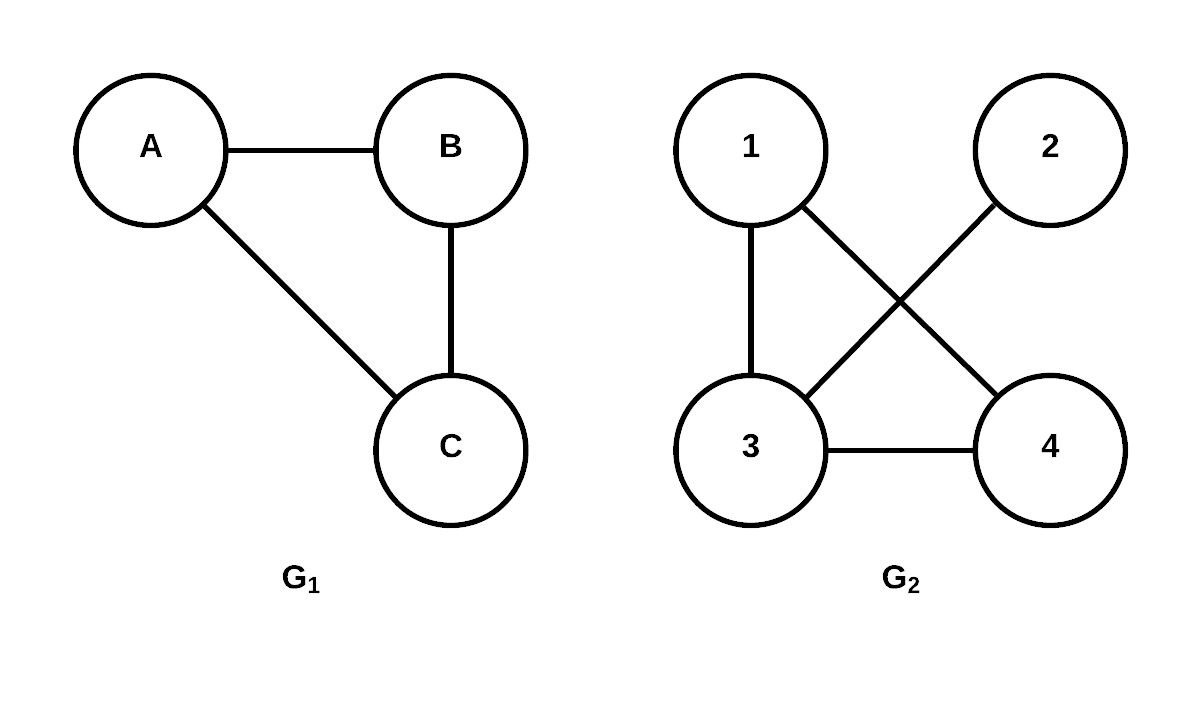
\includegraphics[width=3.5in]{graphs-for-matching-tree.png}
  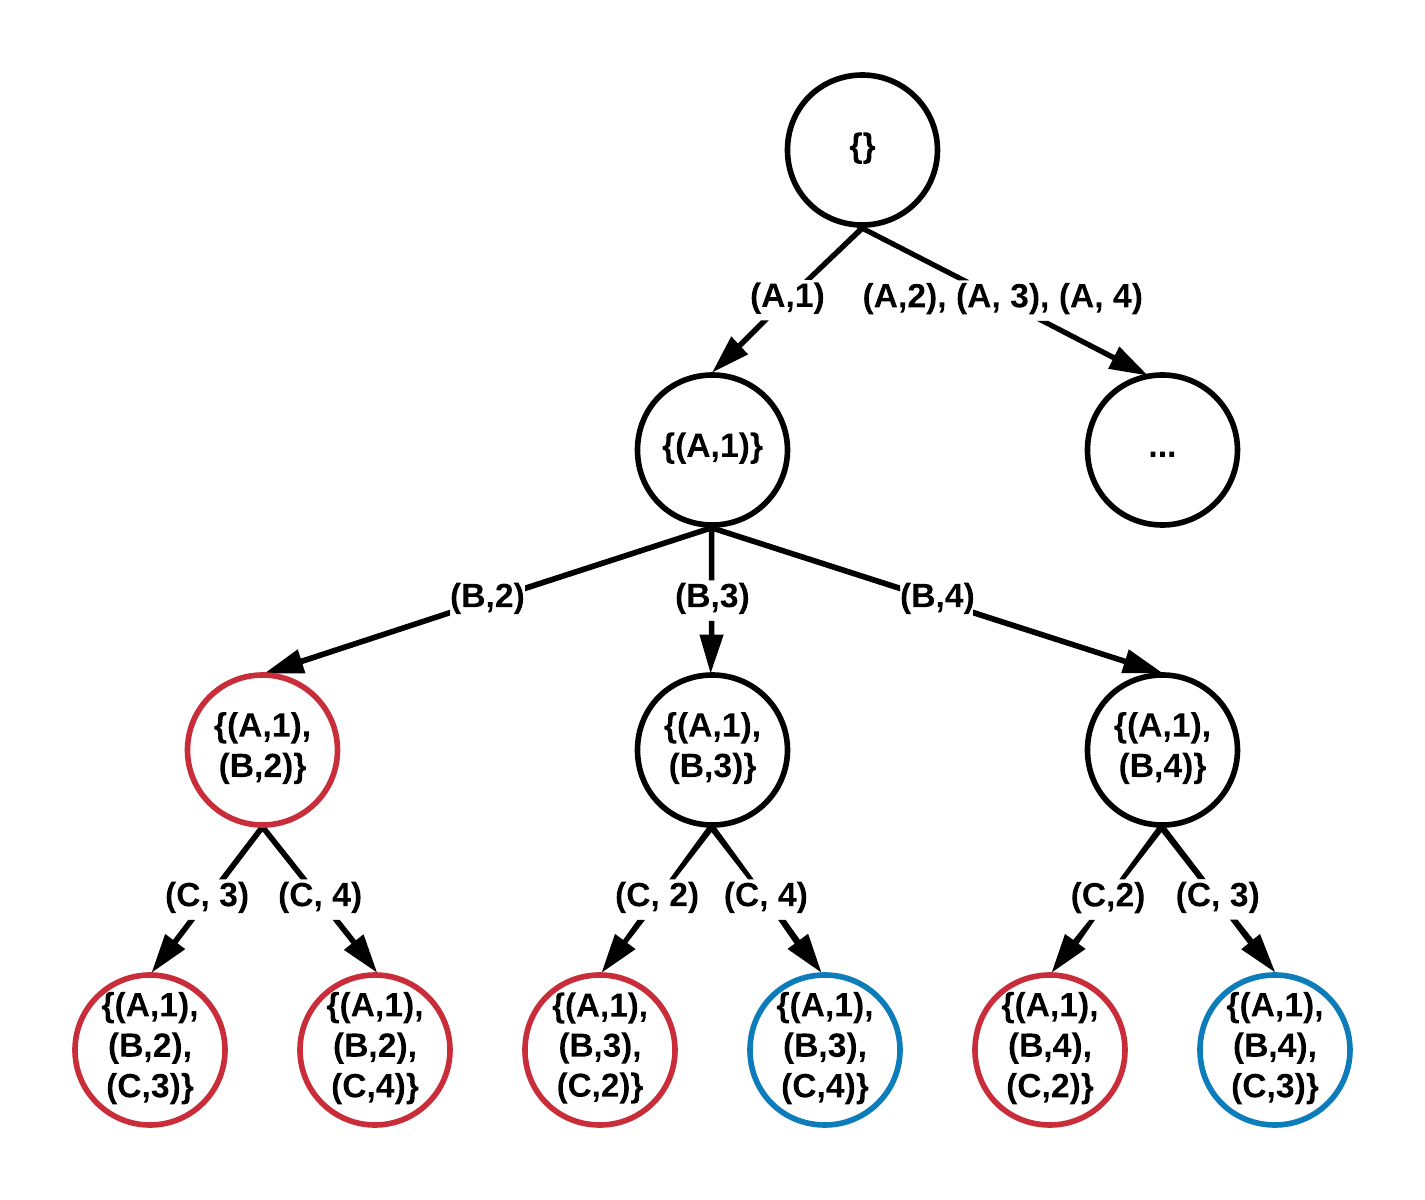
\includegraphics[width=3.5in]{matching-tree.png}
  \caption{Example matching tree.  Blue nodes represent subgraph
    isomorphisms. Red nodes are not adjacency preserving.}
  \label{fig:matching-tree}
\end{figure}

\subsection{Matching Tree}\label{sec:matching-tree}
Our algorithm constructs subgraph isomorphisms by generating
on-line a matching tree and searching through this tree.
%
Consider two graphs $G_1 = (V_1, E_1)$ and $G_2 = (V_2, E_2)$ such
that the vertices of $V_1$ ($V_2$) are totally ordered.
%
We define a \defn{matching tree} from $G_1$ to $G_2$ as a tree with
exactly $|V_1| + 1$ levels or depth, counting from 0.
%
The nodes in the tree represent matchings from
$G_1$ to $G_2$, and the root node represents an empty matching.
%
An edge from a node at level $i$ to level $i+1$ in the matching tree
corresponds to adding a match for the corresponding node at level $i$.
%
A match is a pair of vertices $(u, v)$, where $u \in V_1$ and $v \in V_2$.
%
Each level of the tree matches a single vertex of $V_1$ to a vertex in $V_2$.
%
A node at level $i$ has $|V_2|-i$ children, because at level $i$,
$i$ vertices in $G_2$ have been matched, so there are $|V_2| - i$ vertices left to
match with the vertex from $V_1$ at level $i$.
%
We will also refer to level as depth in the tree.
%
Figure~\ref{fig:matching-tree} shows an example matching tree.


The leaves of the matching tree include all possible subgraph
isomorphisms from $G_1$ to $G_2$, but some leaves are not adjacency
preserving.
%
Some nodes in the tree are also not adjacency preserving, and
furthermore, if a node is not adjacency preserving, none of its
descendants are.
%
This means that an algorithm that searches the tree for an % subgraph
isomorphism could stop when it encounters a node that is not
adjacency preserving.
%
For example, the blue nodes in Figure~\ref{fig:matching-tree} are
valid subgraph isomorphisms.
%
The red nodes are examples of matchings that are not adjacency
preserving.
%
Note that the node representing the matching $\{(A,1), (B,2)\}$ is not
adjacency preserving, and thus all of its descendants are not either,
so they can be pruned. % from the matching tree.

\subsection{Sequential Algorithms for Isomorphism}\label{background::sequential}

%\ur{Motivate. WHy talk about this: 1) bound 2) tools and techniques, framework}

We briefly describe the main ideas behind existing sequential
(sub)graph isomorphism algorithms and present bounds on their run-time
and space use.


A naive sequential algorithm for isomorphism could construct the
entire matching tree, and perform a pre-order traversal over the tree
to find an isomorphism. Such an algorithm requires exponential time
and space and thus is impractical.
%
To achieve better efficiency, a sequential algorithm can construct the
matching tree in an online fashion.
%
To this end, the algorithm maintains its position in the matching tree
by remembering what vertices have been matched, and performs a
pre-order traversal of the matching tree looking for an isomorphism.
%
At a given node, the algorithm either finds an isomorphism and
terminates or computes the children of the node in the matching tree
and recursively searches each child.
%
This approach is the backbone of best known sequential algorithm for
(sub)graph isomorphism including the classic algorithm of
Ullman~\cite{ullman} and the more recent VF2 algorithm by
Foggia~\cite{VF2}, which achieves improved bounds over Ullman's
algorithm.
%
For graphs $G_1 = (V_1, E_1)$ and $G_2 = (V_2, E_2)$ with $n_1$ and
$n_2$ vertices respectively, the sequential online algorithm as
proposed by Foggia requires in the best case time of $\Theta(n_1 \cdot
n_2)$ time, and the worst case time of $\Theta\left(n_2 \cdot
\frac{n_2!}{(n_2-n_1)!} \right)$.
%
The algorithm requires $\Theta(n_2)$ space in the worst
case~\cite{VF2}.
%
Since the algorithm's runtime depends heavily on the structure
of the graphs that are being tested for isomorphism,
the runtime analysis is partitioned into best and
worst case bounds.
%
Proofs for these bounds can be found in
the appendix of the full technical report~\cite{YA-iso-18}.

%%\input{vf}

%\input{alg}
\section{Parallel Algorithm for Isomorphism}\label{sec:par-alg}

To understand the challenges of parallelizing the isomorphism problem,
let us first consider a parallel solution that can be obtained by
directly parallelizing the online sequential algorithm described in
Section~\ref{background::sequential}.
%
Using a classic ``parallel for'', we can write the pseudo-code for
such an algorithm as shown in  Figure~\ref{par-alg}.
%


%\input{fig-par-alg}
\begin{figure}
  \centering

  \hspace*{3mm}
\begin{lstlisting}[language=c, numbers=left]
subgraph_isomorphism (G_1, G_2) =
  // result, initially false 
  R <- (false, {})
  // initial matching, empty  
  M <- \emptyset

  fun search(M) =
    if is_subgraph_isomorphism(M) then
      R <- (true, M)
    else
      children <- Children of M in the matching tree
      parallel_for (u, v) in children:
        if M \cup (u, v) adjacency preserving then
          search(M \cup (u, v))

  // Do search 
  search(M)
  return R
\end{lstlisting}
\caption{Naive Parallel Isomorphism Algorithm Pseudocode}
\label{par-alg}
\end{figure}

Implementing \cd{parallel_for} using nested or fork-join parallelism
as for example implemented in many modern systems such as Cilk, leads
to at least two challenges.
%
These challenges have also been identified
previously~\cite{blankstein}.  We describe  our solution in the rest
of the paper.
%
\begin{itemize}
  \item \textbf{Granularity challenge.} There is no reliable way to
  predict the size of the tree rooted at a given matching, because
  any subtree can be pruned when its root is not adjacency preserving.
  As a result, we may create a very large number of small tasks and the
  structure of the computation is highly irregular.

\item \textbf{Expansion costs.} Since the iterations of the main
  parallel for loop could be executed in parallel, care must be taken
  that they don't lead to race conditions.  This requires making a
  fresh copy of the matching $M$ operated on by each
  iteration. Because the matching $M$ represents $n$ vertices, it has
  size $n$ and thus each copy requires linear space.
  Because we have $n!$ iterations in the worst case, this leads to
  exponential space usage.
\end{itemize}

Our algorithm overcomes the aforementioned challenges by using a lazy
approach to generating parallelism.  The basic idea is to allow each
worker (processor) to ``mimic'' the execution of the sequential
algorithm when running locally but be always ready to generate
parallel work when needed. 
%

In our algorithm, we assume $P$ workers (processors), and a
work-stealing based scheduling algorithm that distributes work among
the workers.


The workers alternate between a work phase, where they do actual work,
and a scheduling phase, where they perform load balancing actions by
responding to steal requests.
%
Each worker maintains a work pool, and on request from the scheduler,
the \defn{victim} worker will migrate half of its work to the
\defn{thief} worker.
%
We assume that the thief demands work only when its work pool is
empty.
%
Apart from this we don't make further assumptions about how
exactly the work stealing scheduler is implemented, e.g., both
sender-initiated or a receiver-initiated approaches could be
employed (e.g.~\cite{EagerLaZa86,MirchandaneyToSt89,Dandamudi97,Dinan+07,acarchra13}).
%

It is an important invariant of the algorithm that it never splits its
work pool unless requested by the scheduler.
%
This means that the uniworker run is essentially the same as the
sequential online algorithm.

\subsection{Data Structures}

Our algorithm uses several data structures, which we call the
frontier, matching, and neighborhood.
%
We describe these data structures and the operations that they
support.

The \defn{frontier} is the work pool maintained by each worker, and is
a set of matches ordered by the depth of the matches.
%
The depth of a match, as defined earlier (Section~\ref{sec:matching-tree}) is the level of
the match in the matching tree, starting from the root (depth $0$).
%
Intuitively, the frontier represents nodes in the matching tree that
need to be explored by the algorithm.
%
The frontier supports \cd{push} and \cd{pop} operations, which
respectively add/remove a largest element to/from the frontier.
%
Crucially, the frontier supports a \cd{split} operation, which splits
it into a prefix and a suffix such that matches in the prefix are less
or equal to those in the suffix.
%
For example, if the frontier is the set $\{(a_1,a_2, 0), (b_1, b_2, 1), (c_1, c_2, 2)\}$,
then the sets $\{(a_1,a_2, 0)\}$ and
$\{(b_1, b_2, 1), (c_1, c_2, 2)\}$ are a valid split,
while the sets $\{(a_1,a_2, 0), (c_1, c_2, 2)\}$
and $\{(b_1, b_2, 1)\}$ are not.

The \defn{matching} data structure is a set of matches, representing a
node in the matching tree.
%
The set of matches corresponds to a partial isomorphism
between $G_1$ and $G_2$.
%

The \defn{neighborhood} data structure is defined for a particular
matching $M$ as a set consisting of the neighbors of all vertices
the domain of $M$, i.e., $\dom{M}$, and the vertices in $G_1$ in $M$.
%
The depth associated with vertices in the neighborhood corresponds
to the depth at which the vertex first entered the neighborhood set.

We define several operations on  matchings and neighborhoods:
\cd{add_match}, \cd{expand}, and \cd{restore}.

The \cd{add_match} operation, whose pseudo-code is given below, takes
a matching $M$, a neighborhood $N$ and a match $(u, v, d)$ and adds 
$(u, v, d)$ to $M$ and adds the neighbors of $u$ in $G_1$ to $N$.
%
\begin{lstlisting}[language=c, numbers=left]
fun add_match(M, N, (u, v, d)) =
  // side effect M and N 
  M <- M \cup (u, v, d)
  N <- N \cup (u, d)
  for u' \in neighbors(u) in G_1 do
    if u' \not\in N:
      N <- N \cup (u', d)
\end{lstlisting}


The \cd{expand} operation, defined below, takes matching $M$,
and a neighborhood $N$, and a new depth $d$ to expand at, and
generates the children
of the node in the matching tree that a matching corresponds to.
%
We compute the expansion by identifying
the smallest labeled node $v_1 \in N$, and returning
a set of matches, matching $v_1$ to each unmatched node in $G_2$.
%
This procedure ensures a consistent exploration of the matching tree,
because it produces the level-by-level structure of the matching tree.
%
Since we try matching the smallest vertex in $N$ to all unmatched vertices in
$G_2$, at every level of the tree, a single vertex from $G_1$ is getting matched.
%
\begin{lstlisting}[language=c, numbers=left]
fun expand(M, N, d) =
  // Projection of M on G_1 and G_2 
  S_1 <- \bigcup_{(u_1, u_2, d) \in M}\{u_1\}
  S_2 <- \bigcup_{(u_1, u_2, d) \in M}\{u_2\}
  v_1 <- smallest vertex in N and not S_1
  // Compute expansion 
  X <- \bigcup_{v_2 \in V_2 \wedge v_2 \not\in S_2}{(v_1, v_2, d)} @\vspace{2mm}@
  return X
\end{lstlisting}

Lastly, the matching and neighborhood support the
\cd{restore} operation, which gives the structures
the ability to backtrack.
%
In sequential search-based isomorphism algorithms, backtracking is
nearly trivial: if a search path is determined not to lead to an
isomorphism, the recursive call stack is unwound
one step at a time, to a point in the
search that offers an alternative search path.
%
In the parallel setting this is more challenging because
the frontier of a worker could be the result
of a split, or could require multiple matches
be removed from the current matching.
%
The \cd{restore} operation, implemented below, takes
a matching $M$, a neighborhood $N$, and a target depth $d$,
and removes all
matches and neighbors from the structures that have a depth
greater than or equal to $d$.
%
The proof of correctness of this operation will be
explored later in the paper, as it is not obvious why
this procedure performs an arbitrary backtrack.
%
\begin{lstlisting}[language=c, numbers=left]
fun restore(M, N, d) =
  // side effect M 
  M <- \{(u, v, d') \in M | d' < d\}
  N <- \{(u, d') \in N | d' < d\}
\end{lstlisting}


\subsection{The Algorithm}

The computation of our algorithm proceeds in steps,
either a \cd{split_step} or a \cd{visit_step}.
%
At any step of the scheduler, a worker can be
executing one of these two operations.
%
\cd{split_step} describes how a worker should split
its work pool, and \cd{visit_step} describes
the computation to be done.
%
Deciding which of these a worker should perform is left
to the scheduler.

Every worker maintains a current matching $M$, neighborhood $N$
and frontier $F$, which are constructed online, and are as
described above.

The \cd{split_step} function takes as arguments a matching $M$,
neighborhood $N$, and frontier $F$. It invokes the frontier's
\cd{split} method to obtain $F_1$ and $F_2$, and returns $F_1$
with $M$ and $N$, and $F_2$ with copies of $M$ and $N$.
%
An example of the \cd{split_step} can be found in Figure~\ref{fig:split-step}.
%
%\hspace{2mm}
%
\begin{lstlisting}[language=c, numbers=left]
fun split_step(M, N, F) =
  // split the frontier and copy M, N 
  (F_1, F_2) <- split(F)
  return ((M, N, F_1),(copy(M),copy(N), F_2))
\end{lstlisting}

\begin{figure}
\centering
  \begin{minipage}[c]{\textwidth}
    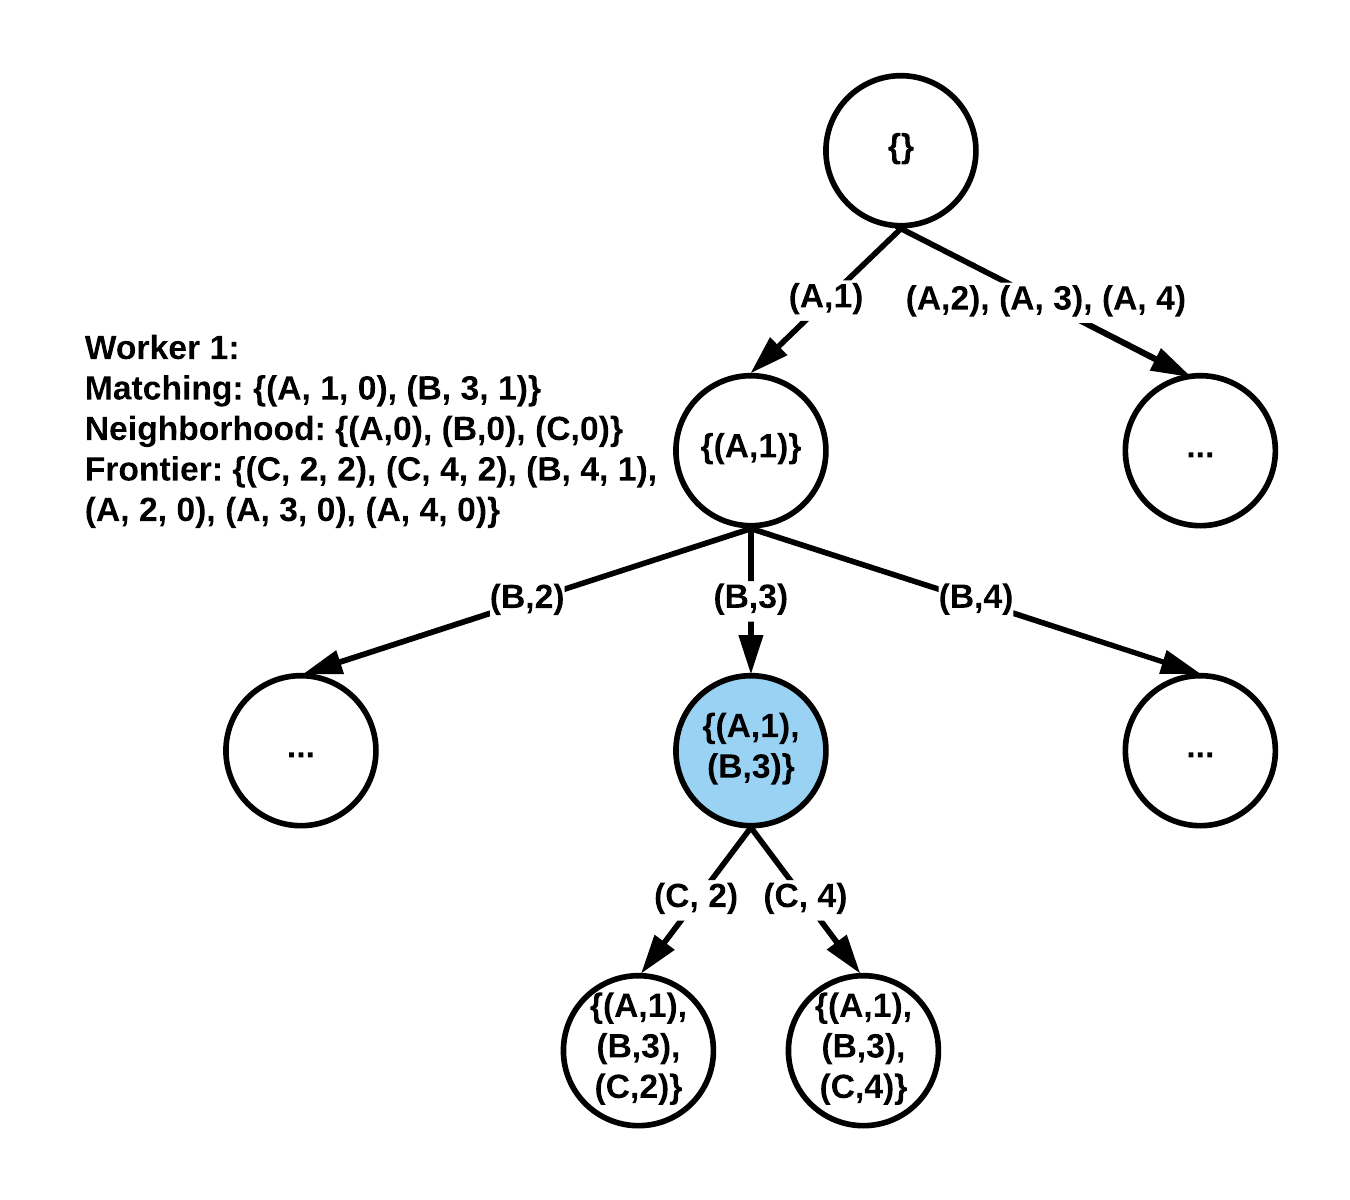
\includegraphics[width=3.5in]{split-diagram-pre.png}
  \end{minipage}
  \begin{minipage}[c]{\textwidth}
    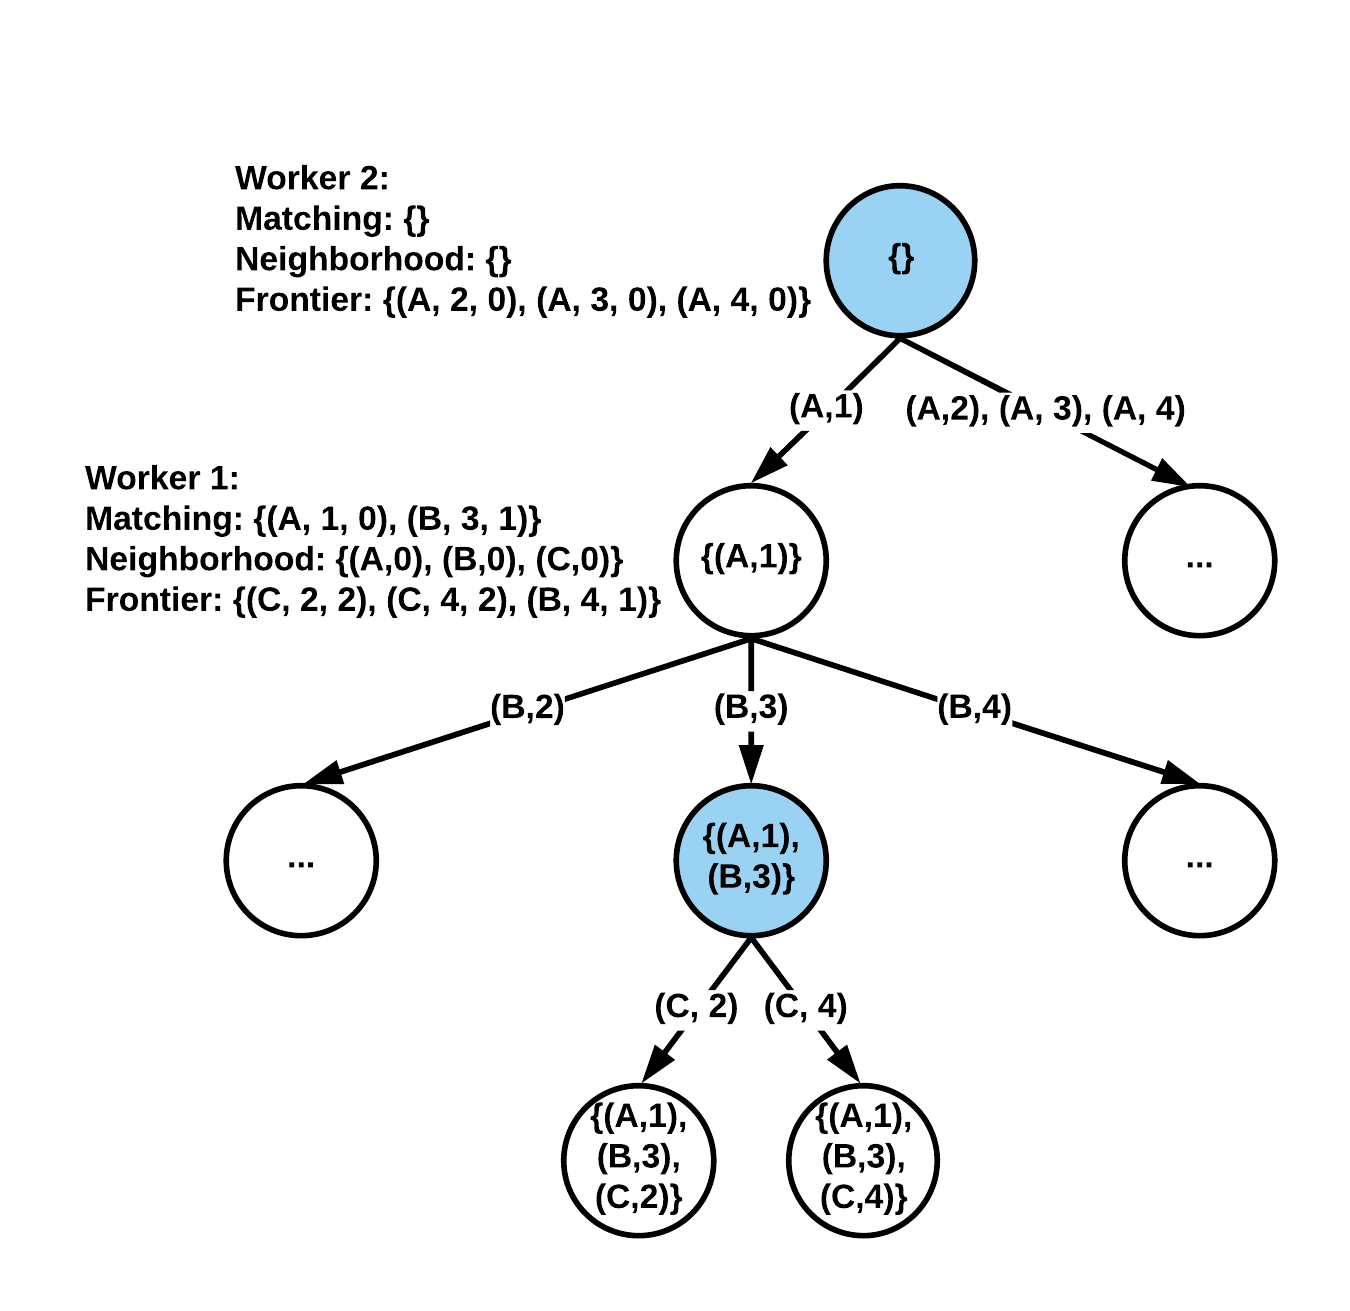
\includegraphics[width=3.5in]{split-diagram-post.png}
  \end{minipage}
  \caption{Example structures from the tree in Figure~\ref{fig:matching-tree}
    for a worker before and after a \cd{split\_step}.
    The highlighted nodes are the processors' current search positions.}
  % These are example states for the tree in Figure~\ref{fig:matching-tree}.}
  \label{fig:split-step}
\end{figure}

If the scheduler requests a worker to
execute \cd{visit_step}, the worker
pops the largest match off of its frontier,
and then uses \cd{restore} to backtrack the
current matching and neighborhood to the right depth.
%
Then, the worker checks to make sure the new match
is adjacency preserving.
%
If so, the worker expands the current matching with
the new match, and adds all the new potential matches
to its local frontier, which concludes the iteration.
%
Code for this function can be found in Figure~\ref{worker-par-alg}.

%\input{worker-par-alg}
\begin{figure}
\begin{lstlisting}[language=c, numbers=left]
// global result, initially false 
R <- (false, {})

// current M, N, and F of a worker 
fun visit_step(M, N, F) =
  // see if another worker succeeded 
  (success, _) <- R
  if success then return R

  // see if there is work to be done 
  if F = {} then return

  // pop off deepest match in F 
  (F', (u, v, d)) <- deepest(F)

  // see if M needs to be restored 
  if d  <= depth(M) then
    restore(M, N, d)

  // verify new M will be adjacency preserving 
  if (M union (u, v, d)) is not adjacency preserving then
    return (M, N, F')

  // destructively update M, N 
  add_match(M, N, (u, v, d))

  // check if success 
  if isomorphism (M) then
    R <- (true, M)
    return

  // add children of new M to frontier 
  F'' <- F' union (expand(M, N, d+1)

  // return state for next iteration 
  return (M, N, F'')
\end{lstlisting}
\caption{Worker Iteration}
\label{worker-par-alg}
\end{figure}


All workers begin with an empty frontier
except for one worker that starts with an initial
frontier to explore.
%
This initial frontier is constructed by taking
the smallest labeled vertex $u \in V_1$ and
constructing the set $\{(u, v, 0) : v \in V_2\}$.
%
All workers halt after an isomorphism has been
found, and if all workers run out of work, then the
algorithm returns false.
%
%% If all workers run out of work before an isomorphism
%% has been found, then the algorithm returns false.

\subsection{Correctness}

The crux of our algorithm is the split and restore operations, which
allow distribution of work and backtracking of search respectively.
%
In this section, we prove a crucial correctness property of
backtracking as implemented by the restore operation.
%
As described earlier this operation is quite simple but its
correctness is not obvious.
%
% The operation works because of several structural properties
% guaranteed by the algorithm and the frontier data structure.
The operation is correct due to structural invariants of the search
tree that we have designed our algorithm and data structures around.
%
In the rest of this section, we state and prove these key invariants,
and use these invariants to prove the correctness of restore.
% prove
% that the restore operation works correctly.


% The crux of our algorithm is the split and restore operations, which
% allow distribution of work and backtracking of search respectively.
% %
% In this section, we prove a crucial correctness property of
% backtracking as implemented by the restore operation.
% %
% The invariants that we observe of the search tree allow us to
% define the frontier and matching data structures and operations
% on these structures appropriately.
%
% These data structures m

\paragraph{Source Paths}
Consider the algorithm's execution on two graphs,
and the matching tree $T$ that it traversed.
%
In $T$, every edge represents a transition
from a \defn{source} matching to \defn{destination} matching.
%
The destination matching is the source matching expanded
with the match that the edge corresponds to.
%
Every match within the frontier corresponds to some
edge within the matching tree, where the source was the
matching that a worker generated the match from.
%
A key invariant that our algorithm upholds is what
we call the \defn{source paths} lemma.

\begin{lemma}[Source Paths]
Let $M$ be the source of the deepest match in a worker's frontier $F$.
%
Let $S$ be the set of sources for every match in $F$.
%
Then $S$ is a subset of the path from $M$ to the root
of $T$.
\end{lemma}

\begin{proof}
This proof will proceed by induction on the iterations
of the scheduler.

In the base case, the initial state of a worker can either have an
empty frontier or the initial frontier
described above.
%
In the first case, the statement holds vacuously
because the frontier is empty.
%
In the second case, the statement holds because the only
source vertex in $F$ is the root node of the matching tree.

For the inductive step, we consider what can occur
in an iteration of the scheduler for a worker.
%
For the inductive step, we consider what actions
the scheduler can request of a worker.
The scheduler can either have the worker run an iteration of \cd{work},
or request the worker to \cd{split}.

First, consider the case a worker performs an step of work.
%
By the induction principle, the worker has a
frontier $F$ that upholds the source paths lemma.
%
Let $M$ be the current matching in tree $T$ and let $m$ be the deepest
match in $F$.
%
We know that $M$ is the source of $m$.
%
The source paths lemma holds for $F$ when $m$ is
removed from $F$, because of the partial ordering invariant of $F$.
%
Once all the children of $M \cup m$ are added to $F$,
the source paths lemma still holds, because now
$M \cup m$ is the source of the deepest node in $F$.
%
The source path in $F$ has been extended to include
$M \cup m$, which concludes this case.

Second, consider the case where the scheduler splits the frontier.
%
By the induction principle, the worker's frontier $F$
upholds the lemma.
%
Let $F_1$ and $F_2$ be the result of the \cd{split} operation.
%
Because \cd{split} returns a prefix and a suffix, both halves maintain
the source paths lemma.
\end{proof}

\paragraph{Correctness of Restore}
To show \cd{restore} correctly backtracks
in the parallel setting we use the invariant
of the source paths lemma described above.
%
The lemma allows the algorithm to limit
the set of possible states to backtrack to.
%
By the source paths lemma, the only nodes
that the algorithm needs to be able backtrack to
are nodes on the path from the current node to the root
of the matching tree.

\begin{theorem}[Correctness of Restore]
  Given a node $a$ at depth $j$ in the matching tree and a depth $i < j$,
  the restore operation returns node $b$ of the matching tree that
  is on the path from $u$ to the root at depth $i$.
\end{theorem}

\begin{proof}
  As a reminder, to \cd{restore} a matching and neighborhood to a target depth
  $d$, we remove all matches and vertices with depth $d'$ greater
  than or equal to $d$.
  %
  We can see from examining the structure of the matching tree that
  if a match $(u, v) \in M$, then for all descendants $M'$ of $M$,
  $(u, v) \in M'$.
  %
  Therefore, $b$ has all of the matches and neighbors whose depth
  is less than $i$.
  %
  By removing all matches and neighbors with depth greater than or equal to $i$
  and keeping all matches with depth less than to $i$,
  \cd{restore} returns a matching representing node $b$.
\end{proof}

Every match in the frontier has depth. Therefore, the algorithm is
always able to generate the matching at the desired depth by using the
\cd{restore} function and a descendant of the desired matching (along
with the appropriate neighborhood).
%
%% On an execution of \cd{split_step}, the algorithm copies its current matching
%% along with half of its frontier, which allows the receiving
%% processor to \cd{restore} the matching it received and begin
%% exploration correctly.


%\input{analysis}
\section{Cost Analysis of Parallel Algorithm}
We analyze the work and space efficiency of our data structures.
%
On a given graph pair $(G_1, G_2)$, let $n_1$ and $n_2$ be the number of
vertices in $G_1$ and $G_2$ respectively, and $n$ be the max of $n_1$ and $n_2$.
%
For work, we show that our algorithm performs asymptotically the same
work as the (online) sequential algorithm.
%
%% This means that on a
%% single core the parallel algorithm performs the same work as the
%% sequential.
%
For space, we show that
the algorithm requires an additional factor $\Theta(p\cdot n)$ more space
than the sequential in the worst case, for a total of $\Theta(p\cdot n^2)$ space overhead.
%
The $\Theta(n)$ factor increase
% The linear factor increase,
% i.e., $\Theta(n)$
comes from the fact that the algorithm maintains a
quadratic size frontier to enable parallelism.
%
The factor $\Theta(p)$ comes from the fact that there can be as many
as $p$ frontiers at the same time.


\paragraph{Frontier.}  
%
The frontier data structure can be implemented by a finger-search tree
that supports
\begin{itemize}
\item  constant-time access to the first (smallest) and the
last (greatest) element of the tree,
\item logarithmic-time split operations.
\end{itemize}
%
There are many such data
structures~\cite{GMPR77,KT96,hinze-paterson-06,chunkedtreesequences} 
and any of these can be used for our bounds.
%\rr{add the citations to the bib file}
%% \ur{Any finger tree should work here really right? The more generic
%%   the better.  For example, Kaplan-Tarjan's catanable sorted lists.}

%% We propose to implement the frontier with a chunked tree style
%% structure, which allows for efficient pop and push to the
%% end of the data structure, as well as supporting
%% an efficient split operation~\cite{chunkedtreesequences}.
%% %
%% This chunked tree structure performs a push and pop operation in
%% amortized $O(1)$ time
%% and a split operation in $O(\log |F|)$ time~\cite{chunkedtreesequences}.
%% %
%% We use the chunked tree structure directly to implement the frontier,
%% and use the bounds proven about the structure for our analysis.

\paragraph{Matching and Neighborhoods.}
We use arrays to represent both the matching and
the neighborhood.
%
For the matching, we maintain an array \texttt{A} such that
for every $(u, v, d)$ match in the matching, \texttt{A[u] = (v, d)}.
%
We use a similar construction for the neighborhood---for
any $(u, d)$ pair in a neighborhood, \texttt{A[u] = d}.
%
With this implementation of the matching and neighborhood,
we can expand a node in the matching tree in $O(n)$ time.
%
Adding a match to the matching takes time relative
to the degree of the vertices in the match.
%
Additionally, we can now bound the \cd{restore} operation's time complexity,
to be $\Theta(n)$.
%% \begin{lemma}
%%   The \cd{restore} operation runs in time $\Theta(n)$.
%% \end{lemma}
%% \begin{proof}
  This can be seen by noting that the length of the arrays
  used to define the matching have length $\Theta(n)$.
  %
  The \cd{restore} operation can make a single pass over
  each of these arrays, and thus take time $\Theta(n)$.
%% \end{proof}
%
The \cd{restore} operation has the same asymptotic cost
as a standard backtrack operation in the serial setting,
so using it instead of a backtrack does not affect the
work efficiency of our algorithm, relative to the sequential algorithm.

\subsection{Space Efficiency}
\begin{theorem}[Space Efficiency]\label{thm:space-efficiency}
  Consider an execution of our algorithm on a pair of (non-empty) graphs
  $G_1$ and $G_2$ with $n_1$ and $n_2$ vertices respectively, and let $n
  = \max(n_1, n_2)$.
  %
  On $p$ processors, our algorithm has space overhead $\Theta(p \cdot n^2)$.
\end{theorem}

\begin{proof}
  Our algorithm incurs space overhead from maintaining
  a matching and neighborhood for each worker, as well
  as maintaining a frontier for each processor.

  Since the representation for the matching and the neighborhood
  uses $\Theta(n)$ space, and every worker has a copy,
  the space overhead due to these structures is $\Theta(p \cdot n)$.

  Now, we show that the space overhead from maintaining the frontier
  is $\Theta(p \cdot n^2)$.
  %
  Consider the matching tree the algorithm explores throughout
  the search.
  %
  By definition of the matching tree, a node can have at most
  $n$ children.
  %
  This implies that at every node in the path from the root
  of the matching tree to the algorithm's current position, the
  algorithm must use $\Theta(n)$ space at each node to the set of possible
  matchings.
  %
  The depth of the matching tree is at most $n$, since
  there are only $n$ nodes that need to be matched before an
  isomorphism is found.
  %
  Since the algorithm needs $\Theta(n)$ space at each node along the path
  from the root of the matching tree to its position, and this
  path can be at most $n$ nodes in length, the algorithm
  uses at most $\Theta(n^2)$ space to store the frontier.
  %
  In the parallel context, every processor can be exploring a path different
  from any other processor, therefore requiring $\Theta(p \cdot n^2)$ space in total.
\end{proof}

\subsection{Work Efficiency}
Consider an execution of our algorithm on a pair of (non-empty) graphs
$G_1$ and $G_2$ with $n_1$ and $n_2$ vertices respectively, and let $n
= \max(n_1, n_2)$.
%
Let $T$ be the matching tree from $G_1$  to $G_2$.
%
We analyze the work of our algorithm by using the \defn{visited tree},
which is the subtree of the matching tree that is visited during the
execution.
%
More precisely, the visited tree is subtree of $T$ that is induced by
the edges of $T$ that were inserted into a worker's frontier during
execution.
%
Throughout, let $N$ be the number of nodes in the matching tree (note
that be the number of edges in the matching tree is $N-1$).


\begin{theorem}[Uni-Processor Work Efficiency]\label{thm:uni-work}
Consider an execution of the \ouralgorithm{} on two graphs with $n_1$
and $n_2$ vertices.
%
Let $N$ be the number of nodes in the matching tree.
%
The algorithm requires   $\Theta(N \cdot \max(n_1, n_2))$ time and work 
on  a single processor.
\end{theorem}

\begin{proof}
  To compute the total work done by our algorithm, we can sum
  the work performed at each node of the visited tree during
  traversal. Let $n = \max(n_1, n_2)$.

  At every node, our algorithm pops a match
  out of the frontier, taking constant time.
  %
  Then, the matching is restored, taking $\Theta(n)$ time.
  %
  Checking whether a matching is adjacency preserving takes at most
  $\Theta(n)$ time, as only the neighbors of the vertices
  in the candidate match need to be verified.
  %
  Both match addition and expansion take $\Theta(n)$ time,
  and the final push onto the frontier takes the same.
  %
  Therefore, the cost per node in the visited tree is $\Theta(n)$.
  %
  Using the cost per node, the total cost of traversing the
  visited tree is $\Theta(N \cdot n + M)$.
  %
  Since the algorithm explores a tree, $M = N - 1$, so
  the final bound of $\Theta(N \cdot n)$ is achieved.
  %
  Since this is a single processor execution,
  there is no additional work performed by the scheduler.
\end{proof}

\begin{corollary}[Uni-Processor Work Efficiency] 
For any two input graphs, the uniprocessor execution of
\ouralgorithm{} is within a constant fraction of the sequential
algorithm.
%
\ouralgorithm{} is therefore work efficient on uniprocessors.
\end{corollary}

\begin{proof}

On a single processor, our algorithm explores the same visited tree
as the sequential algorithm.
%
This is because the the order of exploration our algorithm performs
is the same the sequential algorithm, and there are no split operations
on the uni-processor execution.
%
As Section~\ref{background::sequential} describes, the bounds for the sequential
algorithm are $\Theta(n \cdot N)$.
%
\Ouralgorithm{} achieves the same bounds, as shown in \thmref{uni-work},
and explores the same visited tree, which shows our algorithm is within
a constant fraction of the sequential algorithm.
\end{proof}


% TODO: put in some thetas here?
\paragraph{$P$-Processor Work Efficiency}

We analyze the total (non-idle) work performed by our algorithm by
separating the work performed into three bins:
\begin{itemize}
\item Work done to initialize each worker
\item Work done to explore the visited tree (\cd{visit\_step} function)
\item Work done to split the frontiers (\cd{split\_step} function)
\end{itemize}

\begin{lemma}[Initialization Costs]\label{lem:init-costs}
  The cost of initializing each worker is $\Theta(p \cdot n)$.
\end{lemma}

\begin{proof}
  Each worker maintains a matching of size $\Theta(n)$, therefore
  the work of initializing $p$ states is $\Theta(p \cdot n)$.
\end{proof}

\begin{lemma}[Total Visit Steps]\label{lem:exp-cost}
  Consider the visited tree and let $N$ be the number of nodes.
  The work performed by the \cd{visit\_step} function is $\Theta(N \cdot n)$.
\end{lemma}

\begin{proof}
  In total, $N$ nodes are visited. Each visit, which corresponds to an
  invocation of \cd{visit\_step} requires $\Theta(n)$ work.
  %
  In addition, let $M$ be the number of edges are visited. Each edge visit
  requires a frontier \cd{push} operation in $\Theta(1)$ work.
  %
  Therefore, the total cost from exploring the visited tree is,
  $\Theta(N \cdot n + M)$ and because $M = N - 1$, we have $\Theta(N
  \cdot n)$.
\end{proof}
%

% Now, we must analyze the cost incurred from split operations by the scheduler.
% %
% As shown in theorem~\ref{thm:sched-overhead}, the total overhead from split operations
% is $S \cdot n$.
% %
% Therefore, we must bound the total number of split operations performed through the execution
% of the algorithm.

\begin{theorem}[Number of Splits]\label{thm:split-count}
  The total number of \cd{split} operations performed during execution of the algorithm
  is $\Theta(N)$.
\end{theorem}

\begin{proof}

To analyze the total number of \cd{split} operations performed
during execution of our algorithm, we consider a simple coin based game.
%
In the game, there are active and inactive nodes, and every node has a possibly
empty set of coins.
%
At any step, all active nodes can either recieve a coin, or \cd{split} into
two active nodes (if it has more than one coin), where each active node has half of the original nodes coins.
%
The original node then becomes inactive.
%
The game starts out with a single node, and there is a set amount of coins $c$ that will enter the game.

Imagine we let this game proceed until there are no coins left to enter the game.
%
It is clear that this process will form a tree, with the root being the first node in the game.
%
We can see that there can be at most $c$ leaves in this tree, because if $c$ coins enter the game,
and there can be no splits at a node with only one coin, then there can be at most one leaf left per coin.
%
As this game created a tree, and there are at most $c$ leaves, then the number of internal nodes is $c-1$.
%
Each internal node corresponds to a split operation in the game, which implies that there are most $c-1$ \cd{split}
operations throughout execution of the game.

Now consider the execution of our algorithm mapped to the game.
%
Each coin is an edge from the visited tree, and the active nodes in the game are active workers.
%
Coins are given to nodes when the worker expands its current frontier, and are split when the scheduler
requests a worker to split.
%
Following the result from the coin game, our algorithm can have at most $M$ splits, because the total
number of "coins" to enter the game is $M$.
%
In practice, the number of splits is less than $M$, as edges are consumed by workers as they are visited,
which decreases the total number of coins in the system.
%
Since $M = N - 1$, the total number of splits is upperbounded by $N$.

\end{proof}

\begin{theorem}[Total Split Steps]\label{thm:sched-overhead}
For an execution of \ouralgorithm{}, the total work
spent in \cd{split} is $\Theta(N \cdot n)$.
\end{theorem}

\begin{proof}

Upon a steal request from the scheduler, a worker must
split its frontier and copy its matching.
%
The cost of splitting the frontier is $\Theta(\log(|F|))$, as
discussed previously and shown by~\cite{chunkedtreesequences}.
%
As shown previously, the frontier can be at most size $\Theta(n^2)$,
so the cost of a split operation is $\Theta(\log(n))$.
%
The matching takes $\Theta(n)$ time to copy, since its size is
$\Theta(n)$.
%
As shown in \thmref{split-count}, there are at most $N$ \cd{split} operations,
so the total work spent in \cd{split} is $\Theta(N \cdot n)$.

\end{proof}

\begin{theorem}[$p$-Processor Work Efficiency]\label{thm:multi-work}
Consider an execution of the \ouralgorithm{} on two graphs with $n_1$
and $n_2$ vertices, and let $n$ = $\max(n_1, n_2)$.
%
Let $N$ be the number of nodes in the matching tree.
%
The algorithm requires $\Theta(N \cdot n + p \cdot n)$ work 
on $p$ processors.

\end{theorem}

\begin{proof}

  The total (non-idle) work performed by our algorithm is the sum of the costs
  of initialization, exploration and splitting.
  %
  As shown in Lemma~\ref{lem:init-costs}, the work of initialization is $\Theta(p\cdot n)$.
  %
  The work performed by exploration is $\Theta(N \cdot n)$, as shown in Lemma~\ref{lem:exp-cost},
  and the work performed in splits is also $\Theta(N\cdot n)$, as shown in \thmref{sched-overhead}.
  %
  Therefore the total work performed by our algorithm is $\Theta(N \cdot n + p \cdot n)$.
\end{proof}


\paragraph{Parallelism.}

Our algorithm generates parallelism ``on-demand'' by splitting the
frontier upon a steal request made by another processor.
%
The split operation has logarithmic work and span in the number of vertices.
%
Migration also requires a linear-work copy of the matching but this
operation can be done in parallel in logarithmic span (in the number of vertices).
%
Our algorithm is thus able to generate parallelism quickly on demand.
%
%% \ur{Lying a bit, because there is copy but the copy is
%% cheap because the graphs are small.}

%\input{exp}
\section{Implementation and Experiments}

\subsection{Implementation}
%
We implemented our algorithm by building on several publicly available
pieces of software: 1) VFlib, a fast implementation of the VF2
algorithm for isomorphism~\cite{VF2}, 2) the PASL system for writing
parallel programs targeting modern multicore computers~\cite{acarchra13}, and 3)
the Chunked-Sequence data structure~\cite{chunkedtreesequences}.
%
All of these codes, as well as our extensions, are written in C++.
%
We use the VFLib library functions to implement the graph functions
and the main body of our algorithm.
%
We used the
%primitive functions of
Chunked Sequence library, which
support an efficient finger search data structure, to implement our
frontier data structure and the operations on that data structure.
%
We use the PASL system to implement the parallel distribution of work
among processors.
%
We did not modify any of the of the Chunked
Sequences or PASL code bases, though we did modify the VFLib
implementation to support our algorithm.

\subsection{Optimizations}
Our implementation follows the algorithm description closely but also
includes several optimizations.
%
% TODO: do i need this, responding to comment in paper.
These optimizations are necessary to achieve usable performance,
as without these optimizations a large amount of extra work will
be performed by the algorithm.
%
For example, in our implementation, we extend neighborhoods to include
both graphs.  Specifically, we store the neighbors of the matching in
the second graph in addition to those of the matching in the first
graph.
%
This extensions enables us to implement several search-pruning
heuristics, described in the appendix of technical report~\cite{YA-iso-18}, used by the VF2
algorithm.
%
As another optimization, in our \cd{visit\_step} function, we only add
a match to the frontier if it is  adjacency preserving.
%
This eliminates the need to check if a matching is adjacency
preserving upon popping the match from the frontier and could reduce
the size of the frontier.
%
We note that these optimizations do not change the asymptotic
properties of the algorithm but improve the constant factors.

\subsection{Evaluation}

We evaluated our implementation by using a relatively large graph data
set specifically designed for graph isomorphism.
%
To assess the efficiency and performance, we have compared our
algorithm to the VF2 algorithm~\cite{VF2}, which is a state-of-the-art
algorithm for graph and subgraph isomorphism.

The results show that our algorithm performs quite well and could in
many cases deliver super-linear speedups.
%
This is not surprising, because the algorithm terminates as soon it
finds an isomorphism and thus multiprocessor executions could perform
less work than a uniprocessor one, e.g., if the second processor
quickly finds a matching as it explores a different search path.
%
When reporting our results we therefore report both the average and
the median, because the median is less impacted by the superlinear
speedups.
%
Raw data measurements are presented as tables in the full
technical report~\cite{YA-iso-18}.
%% (Appendix~\ref{app:data}).

\paragraph{Experimental Setup.}
We performed our experiments on a 72-core Dell R930 with four Intel(R)
Xeon(R) E7-8867 v4 processors (18 cores, 2.4GHz and 45MB L3 cache),
and 1Tbyte memory.
%
% Each core is 2-way hyperthreaded giving 144
% hyperthreads. 
%
We compiled our code using g++ 5.4.1 with \cd{-O2} level optimization.
%
To support parallelism, we use the publicly available PASL suite,
which is a C++ library~\cite{acarchra13}.


\paragraph{Data Sets.}
%We have evaluated our results on the publicly available dataset
%offered by Mivia. They have compiled a set of graphs and subgraphs
%called the ARG database that can be used to benchmark both
%graph and subgraph isomorphism algorithms~\cite{argdatabase1}~\cite{argdatabase2}.
%This benchmark set was used by
%the authors of the VF2 algorithm to benchmark their own algorithm,
%as well as in a comparison paper, where they compare their algorithm's
%performance to other popular matching algorithms~\cite{comparisonfive}.
%
We evaluate our results using a benchmarking set for graph and
subgraph isomorphism established by Foggia, Sansone, and
Vento~\cite{argdatabase1}.
%
The database is designed to cover a range of graphs commonly used for
isomorphism testing, including randomly connected graphs, regular and
irregular meshes, and bounded-degree graphs.
%
These graphs are unlabeled and directed.
%
In total the database contains more than 10000 isomorphic graph pairs
and more than 50000 graph pairs that accept a subgraph isomorphism.
%
This data set has been used
in assessing the efficiency of several sequential graph and subgraph
isomorphism algorithms~\cite{argdatabase2,comparisonfive}.
%
This data set contains mainly pairs of isomorphic graphs, rather than
pairs of non isomorphic graphs, which are the ``easy case'' for
search-based algorithms such as ours and our baseline VF2.

%% The reason for this is that the pruning heuristics
%% used by the algorithm are able to quickly detect
%% that the graphs are not isomorphic and exhaust the search
%% space.
%% \rr{is this enough? - about having only isomorphic pairs}

%, which includes a variety of graphs,
%and is meant to be a strong indicator of an isomorphism algorithm's
%performance in real world applications~\cite{argdatabase1}~\cite{argdatabase2}~\cite{comparisonfive}.
%
In our experiments, we consider a subset of the data set consisting of
graphs that are large enough to warrant parallelism. 
%
Specifically, we select graph pairs for which the VF2
algorithm took over one second to complete; we included every graph
pair that took more than one second to run.
%
In addition, we generated new pairs by using the generation software
provided with the data set to increase coverage of full-graph
isomorphism experiments.
%
%% To be specific, we generated a hundred pairs of graphs
%% for each one of the isomorphism pair categories in the appendix.
%% %
%% \ur{How many? What were th parameters used, perhaps in the appendix?}
%% \rr{Is this better? or is more necessary}
%
%
%The authors of the VF2 algorithm have compared their algorithm's performance
%heavily to other existing algorithms and tools, and have concluded that
%their algorithm is one of the top performers in the field of graph matching
%algorithms~\cite{comparisonfive}. We show that our parallelization experiences some slowdown
%on one processor, but on average experienced strong speedup on multiple processors
%over a variety of graph types.
%
%This dataset was meant for the purpose of benchmarking graph isomorphism algorithms,
%and is put together to be a good indicator of real world applications. Within
%this dataset are randomly generated graphs, different dimension meshes with
%varying irregularity, along with graphs of varying bounded degree.
In total, we tested on over 2500 graph pairs from the following
categories:
1) randomly generated graphs,~% (using different edge distributions),
2) bounded degree graphs, with degrees 3, 6, and 9,~
3) regular and irregular meshes in two, three, and four dimensions.
%
%% Our graph data set includes three types of graphs consisting of
%% randomly generated graphs (using different edge distributions),
%% bounded-degree graphs (with degrees 3, 6, and 9), and regular and
%% irregular meshes in two, three, and four dimensions.
%
More details can be found in prior work describing the
data set~\cite{argdatabase1}.

Additionally, for the revised version, we evaluate our algorithm's on
a non-synthetic data set drawn from Damiand et al~\cite{Damiand11} and
Solnon et al~\cite{Solnon15}.
%
These are image datasets, called ``images-PR15'', ``images-CVIU11'',
and ``meshes-CVIU11'' constructed from segmenting images and 3D meshes
of modeled objects.
%
The graphs are undirected and contain both positive and negative
(unsatisfiable) instances.
%
We chose this dataset because it is used by the parallel algorithm for
undirected graphs given by McCreesh et al~\cite{McCreesh15}.
% \ur{dataset does contain, but we don't include no?}
%, unlike in the dataset provided by Foggia et
%al~\cite{argdatabase1}.
%



%% \begin{itemize}
%% \item \textbf{Random Graphs:}
%% These graphs have no regular structure, and each edge is created randomly.
%% There is an edge between two nodes with probability $\eta$, and each edge's
%% distribution is uniform and independent of all other edges.

%% \item \textbf{Bounded Degree Graphs:}
%% These graphs have structure in the degree of all the nodes. In each
%% of these graphs, every node has at most some constant degree. We tested
%% on graphs with degrees of 3, 6, and 9.

%% \item \textbf{Meshes:}
%% We tested on 2D and 4D meshes. The 3D meshes in the dataset
%% did not take VF2 longer than 1 second to complete.
%% %
%% In these meshes, a node is connected
%% to all of its neighbors on the grid that it is in. These graphs are
%% heavily structured, and usually pose a challenge for matching algorithms,
%% due to the structure of the graph~\cite{vf2original}. Additionally,
%% we tested on meshes which were slightly irregular. These meshes had another
%% parameter $\rho$, which determined with which probability a node would
%% connect to a node outside of its neighbors.
%% \end{itemize}

%% \rr{Maybe refactor above to remove irregularity notion}

% TODO: UNCOMMENT OR MOVE TO A FIGURE PAGE
\begin{figure*}
  \centering
    \hfill
    \begin{minipage}[c]{0.22\textwidth}
      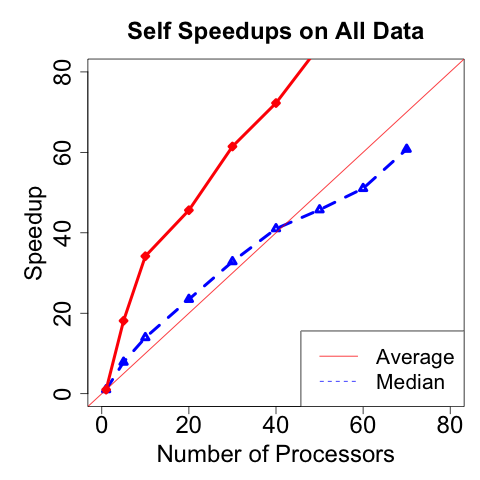
\includegraphics[width=1.0\textwidth]{all-self-speedups-plot.png}
      \caption{\small Self speedup of our algorithm.}
      \label{fig:self-speedup}
    \end{minipage}
    \hfill
    \begin{minipage}[c]{0.22\textwidth}
      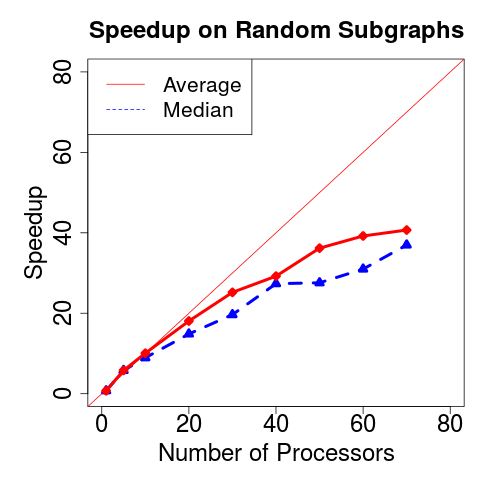
\includegraphics[width=1.0\textwidth]{random-subgraphs-plot.png}
     \caption{\small Subgraph isomorphism with random graphs.}
     \label{fig:speedup-random}
    \end{minipage}
    \hfill
    \begin{minipage}[c]{0.22\textwidth}
      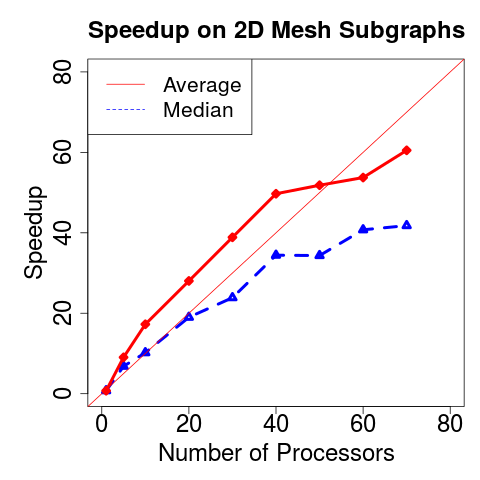
\includegraphics[width=1.0\textwidth]{2d-mesh-subgraphs-plot.png}
     \caption{\small Subgraph isomorphism with random 2D meshes.}
     \label{fig:speedup-mesh-subgraph}
    \end{minipage}
    \hfill
    \begin{minipage}[c]{0.22\textwidth}
      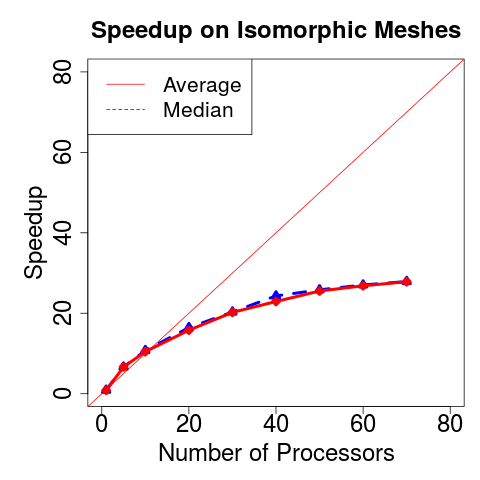
\includegraphics[width=1.0\textwidth]{isomorphic-meshes-plot.png}
     \caption{\small Full graph isomorphism with random 2D meshes.}
     \label{fig:speedup-mesh-fullgraph}
    \end{minipage}
\end{figure*}

%\input{comparison-ciaran}
\begin{table*}[t]
  \centering
  \begin{tabular}{|| c || c | c | c | c | c | c ||}
    \hline
    Dataset & \# Instances & Pattern Sizes & Target Sizes & McCreesh
    Avg Time (s) & Our Avg Time (s) & Improvement \\
    \hline
    \hline
    images-PR15 & 24 Pairs & 4-170 nodes & 4838 nodes & 2.96 & 0.0493 & 60.04x \\
    \hline
    images-CVIU11 & 6424 Pairs & 22-151 nodes & 1072-5972 nodes & 0.649 & 0.1048 & 6.19x \\
    \hline
    meshes-CVIU11 & 2515 Pairs & 40-199 nodes & 208-5873 nodes & 0.532 & 0.0305 & 15.63x \\ % excluding pattern 3
    \hline
    %% Scalefree & 0.258 & 11.633 & 0.022x \\ % excluding some graphs that time us out
    %% \hline
  \end{tabular}
  \caption{Runtime comparison of our algorithm vs McCreesh's algorithm. All times reported
    are run on 72 cores.}
  \label{tab:comparison}
\end{table*}

%\input{util-tab}
\begin{table*}
  \centering
  \begin{tabular}{|c | c |c |c |c |c |c |c| c|}
    \hline
Experiment & Average Slowdown  & \multicolumn{7}{c|}{ Percent Average Utilization of
  Cores }
\\
\hline
& $T_1 / T_s$ & 10 & 20 & 30 & 40 & 50 & 60 & 70
\\
\hline
Subgraph random & 1.39x & 97.1 & 93.7 & 90.1 & 87.1 & 84.5 & 81.9 & 79.5
\\
\hline
Subgraph mesh & 1.33x & 93.8 & 86.8 & 81.6 & 76.9 & 72.7 & 69.9 & 67.1
\\
\hline
Subgraph bvg & 1.37x & 91.8 & 88.6 & 85.3 & 82.8 & 80.4 & 79.6 & 78.0
\\
\hline
Full-graph & 1.14x & 96.2 & 92.1 & 88.9 & 86.2 & 84.4 & 82.3 & 80.8
\\
\hline
\end{tabular}
\caption{Work efficiency and utilization.}
\label{tab:work-and-util}
\end{table*}


% END NOTE ABOVE


%% \begin{figure}
%%   \centering
%%     \begin{minipage}[c]{0.3\textwidth}
%%       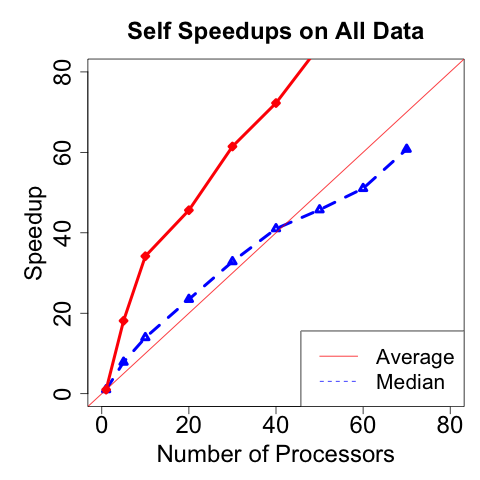
\includegraphics[width=1.0\textwidth]{all-self-speedups-plot.png}
%%       \caption{Self speedup of our algorithm.}
%%       \label{fig:self-speedup}
%%     \end{minipage}
%% \end{figure}

\paragraph{Measurements.}
%
%\ur{Include 1core VF2 run time.}
%\rr{Difficult to, we will see whether it is valid or not}
%
We present the complete set of measurements in several tables in
the appendix of the full technical report~\cite{YA-iso-18}.
%% Appendix~\ref{app:data}.
%
Each line of a table reports the average of the results for a
particular class of graphs being compared, where each class consists of
pairs of graphs of the same kind (random, mesh, etc) with the same
number of vertices and edges.
%
Because of the very large number of graph pairs it is difficult
to visualize this information.
%
We therefore present some of the results as more readily
interpretable speedup plots.
%
% In the speedup plots,
We present both average speedups and the median,
because the median is less sensitive to super-linear speedups that we
observe.

\paragraph{Self-Speedups.}
To evaluate the scalability of our parallel algorithm, we calculated
its self speedup as $T_1/T_P$, where $T_1$ is the uniprocessor run and
$T_P$ is the $P$-processor run.
%
Figure~\ref{fig:self-speedup} shows the average and median
of the self-speedups of our algorithm from all of the experiments.
%
The results
show that our algorithm scales well to high core counts,
and is able to generate plenty of parallelism.


\paragraph{Work-Efficiency Relative to the Sequential Baseline.}  In
Theorems~\ref{thm:uni-work}~and~\ref{thm:multi-work}, we prove that
our algorithm is linear in the size of the search space that is
explored until a (or no) solution is found.
%
This bound is the same as the bounds that state-of-the-art graph and
subgraph isomorphism algorithm such as VF2 achieve.
%
To verify empirically our work-efficiency results, we compared our
algorithm to the VF2 implementation.
%
\tabref{work-and-util} shows in column ``Slowdown'' the slowdown of
single-core execution of our parallel algorithm compared to VF2 for
each three classes of experiments called ``subgraph random'',
``subgraph mesh'', ``subgraph bvg'', and ``full-graph'', which partition (and cover) all our
experimental results.
%
We include more details in the full paper~\cite{YA-iso-18}.


These measurements show that our algorithm is on average between 1.14x and 1.39x
slower than the sequential algorithm on a single core.
%% %
%% Considering that the overheads of thread creation as well as the
%% differences in the data structures and the backtracking operations,
%% this overhead seems very good.
%
Because our parallel algorithms uses different data structures than
the sequential one, we find this difference to be acceptable, because
thread creation overheads alone can lead to such overheads.
%
Specific differences include our frontier data structure (which is not
needed in the sequential algorithm), extra information stored in the
matching data structure,  and the more expensive backtracking
operation needed (restore operation).


%%  in VF2, which is another factor
%% of slowdown.
%% %
%% Lastly, the overheads of thread creation also contribute to the slowdown on
%% a single core.
%% %
%% Considering all of these sources of overhead, the overheads experienced
%% in the experiments seem very good.


\paragraph{Speedups Relative to the Sequential Baseline.}
To compare algorithm to the VF2 algorithm~\cite{VF2}, which is a
state-of-the-art sequential algorithm for graph and subgraph
isomorphism we calculate speedup as $\frac{T_{s}}{T_{P}}$, where
$T_{s}$ is the time taken by the VF2 algorithm on a single core, and
$T_{P}$ is the time taken by our algorithm on $P$ processors.
%
Figures~\ref{fig:speedup-random},~\ref{fig:speedup-mesh-subgraph},~\ref{fig:speedup-mesh-fullgraph}
show the average and median speedups for three different experiments.
%
In our first experiment, we perform subgraph isomorphism for randomly
generated graph pairs and 2D meshes.
%
Figures~\ref{fig:speedup-random}~and~\ref{fig:speedup-mesh-subgraph}
show the speedups.
%
The raw data for these plot is available in the full technical
report~\cite{YA-iso-18}.
%
%% The results show that our algorithm runs between $0.59$x and $0.90$x
%% slower than VF2 algorithm on a single core.
%% %
%% This is expected because our algorithm has to fully generate
%% the set of children for a node, while the VF2 algorithm can
%% construct this set lazily.
%% %
%% The overhead of generating the children and maintaining an
%% explicit stack incurs some slowdown for our algorithm.
%% % \ur{Complete}
%% % Completed
%% %
We observe that as the number of cores increase, the
algorithm delivers increasing speedups.
%
The growth rate of speedup slow down after 40-50 cores, which is
expected because of the memory bandwidth limitations of modern
multi-cores that can be particularly observable in graph algorithms.
%
The utilization of CPU's at 70 cores is 79\%, confirming that the
slowdown in the growth of speedups is not due to lack of parallelism
or other load distribution factors.

%
%
%% Additionally, when self speedup is considered, which is the time taken
%% by the parallel algorithm on one core over the time taken by the parallel algorithm on
%% P cores, our algorithm experiences nearly linear self speedup on a large subset of the
%% tests graphs.
%%

With 2D Meshes, we see that the average and mean speedups are
generally higher, partly because we obtain super-linear
speedups on many inputs.
%
This is quite interesting because these graphs are harder for the
sequential algorithm~\cite{VF2} than random graphs.
%
The reason for this is that our parallel algorithm is able to explore
multiple paths at the same time, and thus can find a subgraph
isomorphism and complete before visiting many other nodes.
%
Because of their regular structure, such graphs tend to have many
different subgraph isomorphisms between them, making it more likely
for our parallel algorithm to find one quickly.



%\ur{Describe in dataset, what is the max degree of meshes?}
%\rr{There is no max degree, there is a parameter $\rho$ which controls
%how likely vertex will connect with another vertex outside of its
%mesh neighbors.}

%
%% They show that our algorithm runs between $0.60$x and $0.84$x slower
%% than VF2 algorithm on a single core, due to the overheads of our
%% parallel algorithm over the sequential one.
%% %



The third experiment, shown in Figure~\ref{fig:speedup-mesh-fullgraph}
shows (full-graph) isomorphism on 2D meshes.
%
For these plots, we used the same generation software as used by Foggia et al~\cite{argdatabase1} to
generate 2D meshes with 4096, 5929 and 7056 nodes.
%% Table~\ref{tab:graph-mesh}.
%% \rr{cite tech report}
%
On these isomorphic meshes we see consistent speedup curves but
compared to subgraph isomorphism experiments, the speedups are lower.
%
We attribute these plateauing speedups to memory bandwidth restrictions,
as our average utilization on isomorphic meshes is 88\% on 70 cores,
which indicates that our algorithm is generating plenty of parallelism.

%% \ur{Reverted back. What was here sounds speculative.  Without data backing it up,
%%   this is going to invite criticism.}
%% ok

%% there is less parallelism than in subgraph isomorphism
%% because the search space is smaller.
%% %
%% We note that the speedup our algorithm achieves depends on the size of the pruned
%% search space represented by the two input graphs.
%% %
%% When the pruned search space is small, such as when the pattern graph is large,
%% the target graph is small, or full graph isomorphism is targeted, then our algorithm
%% has less parallelism to exploit.

%% We also performed experiments with (fully) isomorphic random graphs,
%% the results of which are shown in the technical
%% report~\cite{YA-iso-18}.
%% %% Table~\ref{tab:graph-random}.
%% %% \rr{cite tech report}
%% %
%% %As with  these experiments, we see high amounts of super-linear speedup,

\paragraph{Parallelism and Utilization.}  
%
To confirm that our algorithm generates plenty of parallelism and is
able to keep processors busy, we measured CPU utilization as the ratio
of time spent doing useful work by factoring out time spent idling.
%
\tabref{work-and-util} shows the average
percent utilization of our algorithm on different problem instances
covering our entire data set.
%
The data shows that the utilization is quite good exceeding 78\% in
all instances, except in for the case of ``subgraph-mesh'' instances
it is on the lower side at 66\%.
%
The reason for this is that these instances complete very quickly on
70 cores with a median running time of $0.15$ seconds.


%% Our data shows that even in instances where our speedups plateau our algorithm
%% generates plenty of parallelism, and keep the cores busy.
%% %
%% As our algorithm is able to keep utilizing cores, we attribute plateauing speedups
%% to memory bandwidth limitations of modern multi-core systems.


%% \paragraph{Utilization and Parallelism.}  While our algorithm
%% obtains super-linear speedups in many instances, in other instances, it
%% shows the classic speedup behavior: initially speedups increase
%% linearly with the number of cores, but as the number of cores
%% increase, the rate of increase slows.  We have observed this sort of
%% speedup curves on this machine with essentially all parallel
%% benchmarks that are memory bound (as our algorithm is).  But this
%% still does not answer the question of whether our algorithm does
%% indeed suffer from scalability issues due to lack of parallelism.  To
%% assess, this we measured the utilization of CPU's by measuring the
%% time that cores spent idling or in scheduling.
%% %
%% These measurements show that our algorithm achieves utilization upwards
%% of ? on 70 cores.
%% %
%% algorithm achieves average utilization of greater than 99\% on a
%% single core and upwards of 85\% on 72 cores.

%% This shows that the
%% our algorithm is able to generate a plethora of parallelism and keep
%% cores busy.

\paragraph{Comparison with McCreesh.}  
%
We compare our algorithm to the recent algorithm by McCreesh et
al~\cite{McCreesh15} by using the image data set employed by McCreesh in
their evaluation (described above).
%
McCreesh algorithm cannot be run on our other dataset (the classic
dataset by Foggia et al ~\cite{argdatabase1}), because it assumes
undirected graphs.
%
\tabref{comparison} shows the average 72-core time for McCreesh
algorithm, our algorithm, and the improvement of our algorithm over
the McCreesh algorithm. 
%
The result are averaged over each dataset.
%
In these experiment, we used a total of approximately 9,000 problem
instances and excluded approximately 500, for which either McCreesh's algorithm or
the VF2 algorithm took longer than 100 seconds to complete.
%
The experiments show that our algorithm consistently outperforms
McCreesh's, by as much as 60-fold on first dataset where the target graph
has 4938 nodes.
%
Overall, averaged over all instances, our algorithm is close to a
9-fold faster than McCreesh et al's algorithm.

%
%% \ur{Complete number above.}
%% completed
%% %
%% The set meshes-CVIU11 contains 6 pattern graphs, and 503
%% target graphs.
%% %
%% For one of the pattern graphs, both algorithms performed very slowly,
%% and on some graph pairs with this pattern both algorithms
%% did not complete within 100 seconds.
%% %
%% To avoid skewing the data, we excluded this pattern from our experiments.
%% %
%% We believe that this pattern was a particularly difficult instance for the algorithms,
%% especially ours and VF2, and led to a very large search space to explore.
%
%
%% In the worst case, we perform 6 times better, and 60 times better in the best case.

%
\section{Related Work}
\label{sec:related-work}

\paragraph{Cutting off excess parallelism.}

This study is not the first to propose using cost prediction to
determine when to cut off parallelism.  One approach, developed in
early work in functional programing, uses list size to determine cut
offs~\cite{HuelsbergenLaAi94}. Using list size alone is limited,
because the technique assumes linear work complexity for every
parallel operation.

Another way to handle cost prediction is to use the depth and height
of the recursion tree~\cite{Weening89,PehoushekWe90}. But depth and
height are not, in general, the most direct means to predict the
execution time of subcomputations. In our oracle scheduling, we ask
for either the programmer or compiler to provide for each function a
cost function that expresses the asymptotic cost of applying the
function.

Lopez \textit{et. al.} take this approach as well, but in the context
of logic programming~\cite{Lopez:1996:MGC:241129.241165}. On the
surface, their technique is similar to our oracle scheduling, except
that their cost estimators do not utilize profiling to estimate
constant factors. An approach without constant-factor estimation is
overly simplistic for modern processors, because it relies on
complexity function predicting execution time exactly. On modern
processors, execution time depends heavily on factors such as caching,
pipelining, \textit{etc.} and it is not feasible in general to predict
execution time from a complexity function alone.

\paragraph{Reducing per-task costs.}

One approach to the granularity problem is to focus on reducing
the costs associated with tasks, rather than limiting how many tasks
get created. This approach is taken by implementations of work
stealing with lazy task
creation~\cite{lazy-task-creation,message-passing-ltc,FrigoLeRa98,
  rainey:phd,backtracking-based-load-balancing,SanchezADM}. In lazy
task creation, the work stealing scheduler is implemented so as to
avoid, in the common case, the major scheduling costs, in particular,
those of inter-processor communication. But, in even the most
efficient lazy task creation, there is still a non-negligable
scheduling cost for each implicit thread.

Lazy Binary Splitting (LBS) is an improvement to lazy task creation
that applies to parallel loops~\cite{lazy-binary-splitting}. The
crucial optimization comes from extending the representation of a task
so that multiple loop iterations can be packed into a single
task. This representation enables the scheduler to both avoid creating
closures and executing deque operations for most iterations.
A limitation of LBS is that it addresses only parallel loops whose
iteration space is over integers.  Lazy Tree Splitting (LTS)
generalizes LBS to handle parallel aggregate operations that produce
and consume trees, such as map and
reduce~\cite{BergstromFlRaReSh10}. LTS is limited, however, by the
fact that it requires a special cursor data structure to be defined
for each tree data structure.

\paragraph{Amortizing per-task costs.}

Feitelson \textit{et al.} study the granularity problem in the setting
of distributed computing~\cite{aharoni92arun-time}, where the crucial
issue is how to minimize the cost of inter-processor communication. In
their setting, the granularity problem is modeled as a staging
problem, in which there are two stages. The first stage consists of a
set of processor-local task pools and the second stage consists of a
global task pool. Moving a task to the global task pool requires
inter-processor communication. The crucial decision is how often each
processor should promote tasks from its local task pool to the global
task pool. We consider a different model of staging in which there is
one stage for parallel evaluation and one for sequential
evaluation. 

The approach proposed by Feitelson \textit{et al.} is based on an
online algorithm called CG. In this approach, it is assumed that the
cost of moving a task to the global task pool is an integer constant,
called $g$. The basic idea is to use amortization to reduce the
scheduling total cost of moving tasks to the global task pool. In
particular, for each task that is moved to the global task pool, CG
ensures that there are at least $g+1$ tasks added to the local task
pool. Narlikar describes a similar approach based on an algorithm
called DFDeques~\cite{Narlikar99}. Just as with work
stealing, even though the scheduler can avoid the communication costs
in the common case, the scheduler still has to pay a non-negligable
cost for each implicit thread.

\paragraph{Flattening and fusion.}

Flattening is a well-known program transformation for nested parallel
languages~\cite{Blelloch:1990:CCL:78246.78250}. Implementations of
flattening include NESL~\cite{nesl-implement} and Data Parallel
Haskell~\cite{PeytonJones08}. Flattening transforms the program into a
form that maps well onto SIMD architectures. Flattened programs are
typically much simpler to schedule at run time than nested programs,
because much of the schedule is predetermined by the
flattening~\cite{spoonhower:phd}. Controlling the
granularity of such programs is correspondingly much simpler than in
general. A limitation of existing flattening is that certain classes
of programs generated by the translation suffer from space
inefficiency~\cite{BlellochGr96}, as a consequence of the
transformation making changes to data structures defined in the
program. Our transformation involves no such changes.

The NESL~\cite{nesl-implement} and Data Parallel
Haskell~\cite{PeytonJones08} compilers implement fusion transformation
in order to increase granularity. Fusion transforms the program to
eliminate redundant synchronization points and intermediate
arrays. Although fusion reduces scheduling costs by combining adjacent
parallel loops, it is not relevant to controlling granularity within
loops. As such, fusion is orthogonal to our oracle based approach.

\paragraph{Cost Semantics.}
To give an accurate accounting of task-creation of overheads in
implicitly parallel languages we use a cost semantics, where
evaluation steps (derivation rules) are decorated with work and depth
information or ``costs''.  This information can then be used to
directly to bound running time on parallel computers by using standard
scheduling theorems that realize Brent's bound.  Many previous
approaches also use the same technique to study work-depth properties,
some of which also make precise the relationship between cost
semantics and the standard directed-acyclic-graph
models~\cite{BlellochGr95,BlellochGr96,SpoonhowerBlHaGi08}. The idea
of instrumenting evaluations to generate cost information goes back to
the early 90s~\cite{Sands-thesis,Rosendahl89}.  

\paragraph{Inferring Complexity Bounds.}
Our implementation of oracle scheduling requires the programmer to
enter complexity bounds for all parallel tasks.  In some cases, these
bounds can be inferred by various static analyses, for example, using
type-based and other static analyses
(e.g.,~\cite{CraryWe00,JostHaLoHo10}), symbolic
techniques
%(e.g.,~\cite{Metayer88,Rosendahl89,GoldsmithAiWi07,GulwaniMeCh09}). Our
(e.g.,~\cite{GoldsmithAiWi07,GulwaniMeCh09}). Our
approach can benefit from these approaches by reducing the programmer
burden, making it ultimately easier to use the proposed techniques in
practice.
 


%% \begin{itemize}
%% \item {\em Space-efficient scheduling for parallel, multithreaded computations}, by G. Narlikar~\cite{Narlikar:1999:SSP:930703}.
%% \item {\em Provably Efficient Scheduling for Languages with Fine-Grained Parallelism}, by G. E. Blelloch, P. Gibbons and Y. Matias. Very related: the comment in the third paragraph of the conclusion.
%% %\item {\em Semantics-based parallel cost models and their use in provably efficient implementations}, the thesis %of John Greiner. It has some cost semantics for fork-join parallelism. (see whether it is useful)
%% \item Nesl
%% [Automatic
%%  granularity coarsening based on
%%  profiling~\cite{Chen:2007:STC:1248377.1248396}]
%% \end{itemize}




\section{Related Work}
\subsection{Serial Isomorphism}
There are many serial algorithms for graph and subgraph isomorphism
problems, which are sometimes studied separately because graph
isomorphism is easier~\cite{babai}.
%
Although polynomial time algorithm exists for more specific instances
of graphs, such as planar graphs~\cite{planargraphs}, bounded-degree
graphs~\cite{bounded-degree}, and trees~\cite{trees}, all known
practical algorithms for general graphs require worst-case exponential
time.


Serial graph isomorphism algorithms can avoid exploring the search
space by constructing canonical labelings of the input graphs so as to
match them.
%
Example serial algorithms for graph isomorphism include
Nauty~\cite{nauty-traces} or Bliss~\cite{bliss}.
%

Serial subgraph isomorphism algorithm typically search the solution
space.
%
Central to the effectiveness of these algorithms is a
backtracking algorithm that allows the algorithm to efficiently
back out of a sequence of decisions that lead to a non-solution and
continue searching the rest of the solution space.
%
The first such algorithm was proposed by Ullman in the
seventies~\cite{ullman}.
%
Ullman's algorithm uses matrix operations to perform the search and is
inherently amenable to parallelization.  
%
The algorithm, however, is less time and space efficient---by an
$\Omega(n)$ factor---than more recent algorithms such as ours and
VF2~\cite{VF2} that implement the search more directly.
%
%% For improved efficiency, our algorithm uses a direct implementation of
%% the search as with the VF2 algorithm, rather than relying on matrix
%% operations.
%
%% Our algorithm has the same work efficiency as VF2 but it is parallel.
%a

%% In our experimental evaluation, we use the VF2 algorithm as our
%% baseline, because this algorithm appears to perform best of all known
%% subgraph isomorphism algorithms and because it comes with a large
%% graph data set that can enables rigorous empirical analysis.
%% %

The Ullman and VF2 algorithms, as well as ours, are general-purpose
algorithms that don't take domain knowledge into account (but could
be extended to do so). 
%
One way to use domain knowledge is to assign labels to the
vertices of the graph and matching vertices with the same labels.
%
Depending on the uniqueness of the labels, this approach can vastly
reduce the search space.
%
Owing to the importance of graph isomorphism in applications, this
approach has been well explored.
%
Notable areas of application include databases
(e.g.,~\cite{SZXJ-taming-2008,subgraphdatabase,LHKL-indepth-2012,HLL-turboiso-2013})
and biology and
chemistry~\cite{BGP+subgraph-2013,CGV-performance-2013,subgraphsinchemistry}.
%
Another way to use domain knowledge is to develop heuristics that
help select an order for matching the vertices between two graphs to
improve search time~\cite{ullman-bit-2010}. 
%
For example, a common heuristic is to match vertices with the
highest degree or the least common label
first~\cite{TY-chordality-1984,shier-chordal-1984}.
%
%% Because these techniques either prune the search space or change the
%% order in which it is explored, they remain mostly orthogonal to
%% whether the search is done sequentially or in parallel.
%% %
%% We therefore expect that our algorithm as well as other
%% general-purpose algorithms can be extended to support them.
%% %
%% For example, VF2 algorithm has recently been extended to use such
%% domain knowledge by labeling~\cite{VF3}.
%% %

%% \ur{This should be in the implementation section}
%% \rr{updating this}
%% The authors of the VF2 algorithm have recently presented a new serial
%% algorithm called VF3, which scales to larger graphs~\cite{VF3}.
%% %
%% The main improvements used by the VF3 algorithm are
%% new hueristics for searching, and precalculations of
%% data structures used by the algorithm.
%% %
%% Because VF3 remains fundamentally a search algorithm that explores the
%% large solution space, we expect that its new heuristics can be incorporated
%% into our algorithm.
%% %
%% \rr{how to say this?}
%% As a proof of concept, we implemented the data structure precalculation
%% described by the group, and compared the results to our presented version
%% in Figure~\ref{fig:speedup-optimized}.
%% %
%% We don't see a change in speedup with the optimization,
%% and we believe this is due to the fact that our structure
%% is simple enough that the precomputation doesn't help
%% enough.
%% \rr{Is simple the right word here?}
%% %
%% In the case of VF3, the structure stores more data than in our
%% version, so the precomputation is more effective.

%% \begin{figure}
%%   \centering
%%     %% \begin{minipage}[c]{0.3\textwidth}
%%       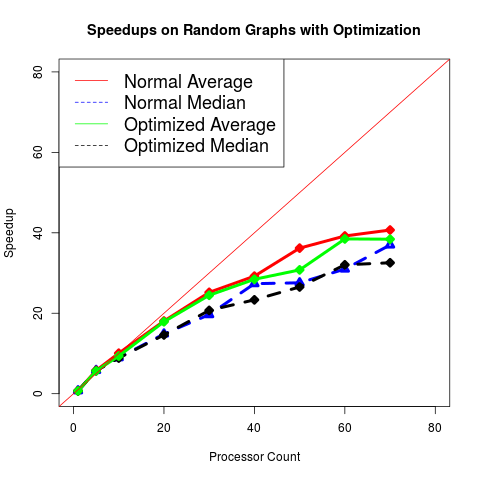
\includegraphics[width=0.3\textwidth]{optimized-plot.png}
%%       \caption{Speedup of our algorithm using the state structure optimization.}
%%       \label{fig:speedup-optimized}
%%     %% \end{minipage}
%% \end{figure}



\subsection{Parallel Graph Isomorphism}
There has been some work on parallel full-graph isomorphism algorithms
by using GPUs to accelerate sequential algorithms such as
Ullman's~\cite{ullman} and canonical-labeling
algorithms~\cite{gpuiso,gpu-canon-forms}.
%
Although these papers do not consider general-purpose hardware such as
multicores, the result could probably be extended to do so.
%
The parallel algorithms based on Ullman's algorithm, however, would
not lead to work efficient algorithms due to its inherent work
inefficiency.

In contrast to parallel graph isomorphism, there has been relatively
little work on the harder problem of parallel subgraph isomorphism.
%
An unpublished class project (at MIT) by Blankstein and Goldstein,
consider the subgraph isomorphism problem on general graphs and
present a parallel search algorithm~\cite{blankstein}.
%
%% The authors implement their algorithm on multicores using the VFLib as
%% a base~\cite{blankstein} and the C++ language with Cilk
%% primitives~\cite{blumofe96,frigolera98}.
%
The authors encounter the challenges discussed in
Section~\ref{sec:par-alg}, including the memory blowup, backtracking,
and scheduling problems.
%
They propose a heuristic that decides whether a branch should run in
parallel or not, and an operation called a conditional copy to curb
the memory blowup.
%
The conditional copy operation preserves the semantics of the
sequential algorithm but allows for an object to be copied if and only
if it was the result of a steal operation under a work stealing
scheduler.
%
As the authors also point out, the heuristic may or may not work
depending on the graph, leading to unpredictable performance, and
making it difficult to establish work-efficiency bounds.
%
% TODO: need more?
McCreesh et al~\cite{McCreesh15} present a constraint based search
algorithm, which explores a search tree in a parallel depth first
fashion, while using supplemental graphs to prune the search space. 
%
As in Blankenstein's approach (\secref{par-alg}) they use speculation
to parallelize the search loop and present no efficiency or
parallelism bounds. They show empirically that their algorithm can
perform well compared to VF2 on their data set.
%
Kimmig et al present a parallel algorithm for subgraph enumeration
problem based on the serial RI algorithm~\cite{BGP+subgraph-2013},
which targets biological data and uses labeling heuristics;
%
the authors do not present bounds on efficiency or parallelism.

%% In an separate line of work, some researchers have worked on
%% implementing Ullman's original algorithm~\cite{ullman} in GPUs.
%% %
%% Because Ullman's algorithm uses matrix operations, it is amenable to
%% parallelization on GPUs~\cite{gpuiso}.
%% %
%% Ullman's algorithm, however, is less efficient---by a linear
%% factor---in time and space than ours.
%% %
%% There has also been work on accelerating the computation of canonical
%% labeling methods for the (full)-graph isomorphism
%% problem~\cite{gpu-canon-forms}.
%% %


%
Raman et al~\cite{subgraphdatabase} present a parallel subgraph
isomorphism algorithm tailored to queries in graph
databases.
%
As in our work, they start with a search algorithm but they point out
that due to the depth-first nature of such algorithms, parallelization
is challenging.
%
They then present a breadth-first approach and evaluate in the
specific domain of certain graph databases.
%
The problem with a breadth-first search approach is that it can require a
lot of space, because each level of the search space could be
exponentially large in the size of the graphs.
%
Raman et al show that this problem is less of a concern in the graph
databases they considered, because the vertices are labeled (sometimes
uniquely) and thus the search space can be pruned aggressively.
%
A secondary problem with breadth-first search is that processors must
synchronize at every level of the graph, which has detrimental effects
on scalability and
locality~\cite{endo1997scalable,siebert2010concurrent,flood2001parallel,congkokrlesa08,pdfs-15}.
%
In our work, we consider the general problem of unlabeled graphs, and
show that the classic depth-first approach to
isomorphism can be parallelized effectively.
%

There has been recent interest it in parallelizing backtracking search
algorithms in distributed systems. Abu-Khzam et
al~\cite{S+scalable-2009} present techniques based on indexing of the
search tree and Schmidt et al~\cite{F+scalable-2015} present
techniques for maximal clique enumeration.
%
They don't consider graph isomorphism problem but have excellent
discussions of the challenges that parallel search-state algorithms
must solve.


\subsection{Lazy splitting}
%
The search-based algorithm for subgraph isomorphism that explores the
space of solutions appears to be a naturally parallel algorithm,
because the order in which the search is performed does not matter.
%
As described here (Section~\ref{sec:par-alg}) and also observed by other
researchers~\cite{blankstein,subgraphdatabase}, the algorithm resists
efficient parallelization.
% when
%
% using standard nested-parallelism
%primitives such as fork-join, parallel for, etc.
%
%The primary reason for
One reason for this is the difficulty of backtracking.
%
Another reason is that the search is a highly irregular and there is
no easy way to determine a priori how much computation a parallel task
will perform.
%
As a result, the algorithm can generate excess parallelism, which can
lead to significant run-time burden, because creating parallel tasks
requires linear work and space.
%

This is an instance of the classic granularity problem that arises in
many parallel algorithms and have been studied quite extensively.  One
potentially promising approach called {\em lazy
  splitting}~\cite{mohr-lazy-1991,GoldsteinScCu95,goldstein96,frigolera98,backtracking-based-load-balancing,tcvb-lazy-scheduling-14}
has received more attention especially recently, as parallelism has
grown from traditional scientific application benchmarks to wider
areas of computer science.
%
The basic idea behind lazy splitting is to postpone creation of
threads until there is concrete demand for parallelism, e.g., workers
are idling.
%
%% Although some of these techniques have entered into production systems
%% and have led to improved performance overall, significant challenges
%% remain. For example, when parallel constructs are nested, many of
%% these approaches have been shown to fail in controlling overheads for
%% certain classes of programs~\cite{tcvb-lazy-scheduling-14}.
%% %
%%
Our algorithm uses the lazy splitting technique by splitting the
frontier lazily upon a steal request. In our algorithm splitting the
frontier requires logarithmic time, and thus does not adversely impact
the availability of parallelism.
%
Furthermore, because the frontier is
split evenly in half, the algorithm guarantees balanced distribution
of the current work.


%% One fundamental challenge in lazy scheduling is determining when to
%% create parallelism. Many of the existing approaches rely on local
%% heuristics, e.g., if the local work pool is sparsely populated, then
%% parallelism should be created.
%% %
%% Unfortunately, such heuristics can fail and sometimes increase the
%% span significantly, as remarked by Tzannes et al~\cite{tcvb-lazy-scheduling-14}.
%% %
%% A general problem with lazy scheduling is thus establishing bounds.
%% %
%% For example, Tzannes et al~\cite{tcvb-lazy-scheduling-14} authors only
%% give a bound on the execution time for the case of a single parallel
%% loop taken in isolation.


%
%\section{Conclusion}

%% \section{Future work}
%% \label{sec:conclusion}

%% In this work, we have implemented oracle scheduling on top of a
%% work-stealing scheduler.  It would be interesting to also investigate
%% the use of other schedulers, \textit{e.g.}, schedulers based on a
%% shared queue, and scheduler that improve data
%% locality~\cite{AcarBlBl02}.  We could also try to apply this technique
%% to a distributed setting, where spawning parallel tasks not only
%% requires the migration of code but also that of data, which can be
%% very costly.

%% %\uremark{The depth discussion comes out of the blue. Explain a bit
%% %  more perhaps.}

%% In our implementation, we have fixed $\coff$
%% to be a constant value, but we could try to dynamically
%% adjust it. However, there is a major difficulty: obtaining
%% accurate estimates for the raw depth is much harder than for
%% the raw work. Indeed, for raw work it suffices to measure the
%% time taken by a sequential execution of a task. There is no
%% such easy way to measure the raw depth of a program.

%% %\uremark{Transition.}
%% To realize the oracle, we have assumed that the programmer
%% would provide complexity functions explicitly.
%% This seems to be a reasonable assumption in general.
%% However, for particular application domains it is possible to
%% use static analysis techniques to infer those complexity
%% bounds. We could also use dynamic analysis, in particular
%% machine learning techniques, for automatically guessing the 
%% shape of the complexity function.

%% We have also assumed that the complexity functions could be
%% implemented in constant time. In the context functional data
%% structures, this often requires storing size information in data
%% structures. Fortunately, this can be achieved at a small cost with
%% compiler support, as done for example in other
%% work~\cite{Hermenegildo-garcia-95}.  


%************************
\begin{comment}
We have presented a general solution to a fundamental problem
arising in parallel computations, namely the granularity problem.
The key contribution of this paper is the observation that 
complexity cost functions provided by the programmer are sufficient
for making good run-time decision about whether to exploit or ignore
the parallelism available in a program.
We have argued for the interest of our approach both
through the presentation of theorems establishing bounds
on the costs of scheduling and through experiments reporting
significant speedups compared with other scheduling techniques.
\end{comment}

\section{Conclusion}

In this paper, we propose a solution to the granularity-control
problem.  We prove that an oracle that can approximate the sizes of
parallel tasks in constant time within a constant factor of accuracy
can be used to reduce the task creation overheads to any desired
constant fraction for a reasonably broad class of computations.  We
describe how such an oracle can be integrated with any scheduler to
support what we call oracle scheduling.  We realize oracle scheduling
in practice by requiring the programmer to enter asymptotic complexity
annotations for parallel tasks and by judicious use of run-time
profiling.  Consistently with our theoretical analysis, our
experiments show that oracle scheduling can reduce task creation
overheads to a small fraction of the sequential time without hurting
parallel scalability.


\section{Conclusions}

This paper presents and evaluates a parallel algorithm for the graph
and subgraph isomorphism problems.
%
Compared to state the art sequential algorithm for isomorphism, our
algorithm is asymptotically work efficient.
%
It also performs reasonably well in practice, exhibiting only a small
slowdown to the carefully engineered VF2 algorithm.
%
Our algorithm performs reasonably well on high core counts on both the subgraph
and graph isomorphism problems, and is agnostic to the graph
structure, which makes it potentially suitable for a large variety of
graphs.
%
The technical contributions behind the algorithm include the
techniques for ensuring that local search operations remain efficient,
while also enabling splitting of work for parallel execution.
%
This is achieved by using a splittable frontier data structure and a
search algorithm that can backtrack efficiently without using
additional space.
%
These results suggest that parallel search strategies could by
succesfully applied to NP-complete and NP-hard  problems.



%% Our results show that the graph isomorphism and subgraph isomorphism
%% problems can be efficiently parallelized, and these parallel solutions can
%% be used
%% by various applications that use graph matching.
%% %
%% Additionally, we believe that our approach of using lazy splitting
%% to search a space can be applied to problems other than isomorphism.
%% %
%% % TODO: add more details about generalizing approach and space complexity stuff
%% %
%% Our code is available publicly at this link (insert).
%% \rr{Update the conclusion}


\bibliographystyle{plain}
\bibliography{../bibliography/main,../bibliography/new,../bibliography/leiserson,../bibliography/iso,./chunked}



%% Uncomment for full tech report
% \newpage
% \input{appendix}

\newpage
% \input{ad-appendix}

